\chapter{Конформная теория поля}
\label{cha:cft}

Подробное изложение \cite{difrancesco1997cft}. 

\section{Общие свойства}
\label{sec:cft-general}
Алгебра Вирасоро. Представления алгебры Вирасоро. Модулярная инвариантность.

\section{Модели Весса-Зумино-Новикова-Виттена}
\label{sec:wzw}
Связь с аффинными алгебрами Ли.
Конформные вложения и недиагональные модулярные инварианты. 



%\usepackage{verbatim} 
\newenvironment{comment}
{\par\noindent{\bf Для заинтересованных читателей}\\}
{\\\setlength{10cm}\\\hfill$\scriptstyle\blacksquare$\par}


\begin{abstract}
Примерный текст доклада на семинаре кафедры ФВЭиЭЧ по работе ``Recursive algorithms, branching coefficients and applications''.
\end{abstract}

\section{Постановка задачи}
\label{sec:task}

Здравствуйте!
Сегодня я хочу рассказать о работе ``Рекуррентные алгоритмы, коэффициенты ветвления аффинных алгебр
Ли и приложения''. В этой работе мы решали следующую задачу.

Даны две аффинные алгебры Ли $\mathfrak{a}\subset \mathfrak{g}$. Аффинные алгебры Ли --- это особый
класс бесконечномерных алгебр, которые строятся из конечномерных (полу)простых алгебр Ли, как
центральные расширения алгебр петель. Более подробное определение будет дано позже. Неприводимое
представление $L^{(\mu)}_{\mathfrak{g}}$ аффинной алгебры $\mathfrak{g}$ со старшим весом $\mu$
может быть разложено на представления подалгебры $\mathfrak{a}$. Наша задача --- придумать
практический алгоритм вычисления коэффициентов этого разложения. Конечно же эта задача уже решалась,
например, существует способ решения ``в лоб'', требующий построения всех представлений и различные способы,
которые работают для частных случаев, например, многое упрощается в физически интересном случае
конформных вложений. Мы предлагаем общий метод, но иллюстрировать его будем как-раз физическими
примерами конформных вложений.

Я начну с физической мотивации этой задачи в двумерной конформной теории поля, напомню некоторые
факты из теории представлений аффинных алгебр Ли, кратко опишу предложенное нами решение проблемы и
расскажу про физические примеры в нашей статье.

\section{Физическая мотивация}
\label{sec:physics}

\subsection{Напоминание про двумерную конформную теорию поля}
\label{sec:CFT}

Конформное преобразование --- это преобразование, меняющее только масштаб у метрического тензора:
\begin{equation}
  \label{eq:10}
  g'_{\mu\nu}(x')=\Lambda(x)g_{\mu\nu}(x)
\end{equation}

Конформная теория поля --- это теория поля, обладающая инвариантностью относительно этих преобразований.

В теории струн двумерная конформная теория поля описывает динамику на мировой поверхности, а в
теории критических явлений --- фазовые переходы в двумерных системах.

%% В $D$-мерном случае генераторы у таких преобразований следующие:
%% \begin{align}
%%   \label{eq:1}
%%   & M_{\mu\nu} \equiv i(x_\mu\partial_\nu-x_\nu\partial_\mu) \,, \\
%%   &P_\mu \equiv-i\partial_\mu \,, \\
%%   &D \equiv-ix_\mu\partial^\mu \,, \\
%%   &K_\mu \equiv i(x^2\partial_\mu-2x_\mu x_\nu\partial^\nu) \,,
%% \end{align}
%% 
На двумерной мировой поверхности удобно ввести комплексные координаты $z,\bar{z}$. 
В двумерном случае существует бесконечное число локально-конформных преобразований.
Это легко можно увидеть из условия конформности преобразований, так как в двумерном случае это
условие эквивалентно уравнению Коши-Римана для голоморфных функций ($\partial_{\bar z}w(z,\bar
z)=0$).

Таким образом локально-конформные преобразования находятся в однозначном соответствии с множеством
всех аналитических функций $w(z)$ на плоскости.  

Глобальные конформные преобразования имеют вид $f(z)=\frac{az+b}{cz+d},\; ad-bc=1$. 

Рассмотрим инфинитезимальные преобразования $w(z)=z+\epsilon(z),\quad
\epsilon(z)=\sum_{-\infty}^{\infty}c_nz^{n+1}$. 
Тогда для бесспинового поля $\phi(z,\bar z)$ верно следующее: $\phi'(z',\bar z')=\phi(z,\bar z)$,
$\delta\phi=-\epsilon(z)\partial\phi-\bar \epsilon(\bar z)\bar \partial \phi=\sum_n(c_n L_n\phi+\bar
c_n\bar L_n\phi)$, где $L_n=-z^{n+1}\partial_z,\quad \bar L_n=-\bar z^{n+1}\partial_{\bar z}$

Мы видим, что в классической теории алгебра конформных преобразований --- это алгебра Витта, которая
порождается генераторами $\{L_n, n\in \mathbb{Z}\}$ --- модами разложения оператора энергии-импульса $T$, с
коммутационными соотношениями
\begin{equation}
  \label{eq:2}
  [L_m,L_n]=(m-n)L_{m+n}
\end{equation}
При квантовании возникает конформная аномалия, что соответствует центральному расширению алгебры (то
есть появлению центрального заряда $c$). В коммутационные соотношения надо добавить член
$\frac{c}{12}(m^3-m)\delta_{m+n,0}$. В результате получаем алгебру Вирасоро.

(Про тензор энергии-импульса:
$x^{\mu}\to x^{\mu}+\epsilon^{\mu}\Rightarrow \delta S=\int d^2 x
T^{\mu\nu}\partial_{\mu}\epsilon_{\nu}=
\frac{1}{2}\int d^2 xT_{\mu}^{\mu}\partial_{\rho}\epsilon^{\rho}$
В двумерной конформной теории поля тензор энергии-импульса бесследовый).

Поля теории $\phi(z,\bar z)$ должны преобразовываться определенным образом при конформных преобразованиях.
Оказывается, что все поля группируются в конформные семейства, в которых есть одно примарное поле
\begin{equation}
  \label{eq:3}
  \begin{split}
    \phi_{\Delta,\bar \Delta}(z,\bar z)\underset{
      \genfrac{}{}{0pt}{}{z\to w(z)}
        {\bar z \to \bar w(\bar z)}
    }
    {\longrightarrow} \left(\frac{dw}{dz}\right)^{\Delta}\left(\frac{d\bar w}{d\bar
        z}\right)^{\bar\Delta}\phi_{\Delta,\bar \Delta}(w(z),\bar w(\bar z))\\
    L_n \phi=0,\quad n>0\\
    L_0 \phi=\Delta \phi\\
  \end{split}
\end{equation}
$\Delta, \bar \Delta$ называются конформными размерностями поля.
Все остальные поля называются вторичными и получаются из примарного действием операторов $L_{-n}$:
\begin{equation}
  \label{eq:67}
  L_{-n_1}L_{-n_2}\dots \phi_{\Delta}
\end{equation}
Все поля в теории оказываются суммами произведений элементов мультиплетов алгебры Вирасоро.

При некоторых дополнительных предположениях двумерную конформную теорию можно построить и решить
полностью, если определен набор примарных полей и конформных размерностей. 

Существуют различные подходы к аксиоматизации двумерной конформной теории поля. В общем случае нам
не нужно знать действие, если мы полный знаем набор примарных полей и операторные разложения их
произведений. 

В том случае, если в теории конечное число примарных полей, такая теория называется минимальной.
Кроме того, теории классифицируются по значениям центрального заряда $c$. Теории с рациональным
центральным зарядом называются рациональными. Оказывается, что все такие теории могут быть получены
факторизацией так называемых моделей Весса-Зумино-Новикова-Виттена.

\subsection{WZW-модели}
\label{sec:wzw}

WZW-модели обладают дополнительной симметрией. Алгебра токов в них --- это алгебра Каца-Муди
(аффинная алгебра Ли $\mathfrak{g}$), полная киральная алгебра --- полупрямое произведение
$Vir\ltimes \mathfrak{g}$, примарные поля преобразуются по неприводимым представлениям алгебры $\mathfrak{g}$.

Сейчас я поясню, что все это значит и как строятся такие модели.

Модели Весса-Зумино-Виттена можно строить начиная со следующего действия:
\begin{equation}
\label{eq:4}
  S=S_0+k\Gamma
\end{equation}
где $k$ - целое.
Здесь $S_0$ --- действие нелинейной $\sigma$-модели.
\begin{equation}
  \label{eq:5}
  S_0=\frac{1}{4a^2}\int_{S^2} d^2x\; Tr (\partial^{\mu}g^{-1}\partial_{\mu}g),
\end{equation}
где $a^2>0$ - положительный параметр, $g(x)\in G$ - поле со значениями в группе $G$, которую мы
будем считать полупростой. Действие задается на комплексной плоскости с бесконечностью, которая
топологически эквивалентна 2-сфере.

В нелинейной $\sigma$-модели конформная инвариантность теряется на квантовом уровне.
Голоморфный и антиголоморфный токи не сохраняются по отдельности.
Поэтому мы добавляем член Весса-Зумино $\Gamma$ к действию
\begin{equation}
  \label{eq:73}
\Gamma= - \frac{i }{24\pi} \int_{B}\epsilon_{ijk} Tr\left(
    \tilde g^{-1}\frac{\partial \tilde g}{\partial y^i}
      \tilde g^{-1}\frac{\partial \tilde g}{\partial y^j}
      \tilde g^{-1}\frac{\partial \tilde g}{\partial y^k}\right) d^3y
\end{equation}
Он определен на трехмерном многообразии $B$, ограниченном исходным двумерным пространством.
Через $\tilde{g}$ мы обозначили продолжение поля $g$ на $B$. Такое продолжение не единственно. В
компактифицированном трехмерном пространстве компактное двумерное многообразие разделяет два
трехмерных многообразия.
\begin{figure}[h]
 \centering
  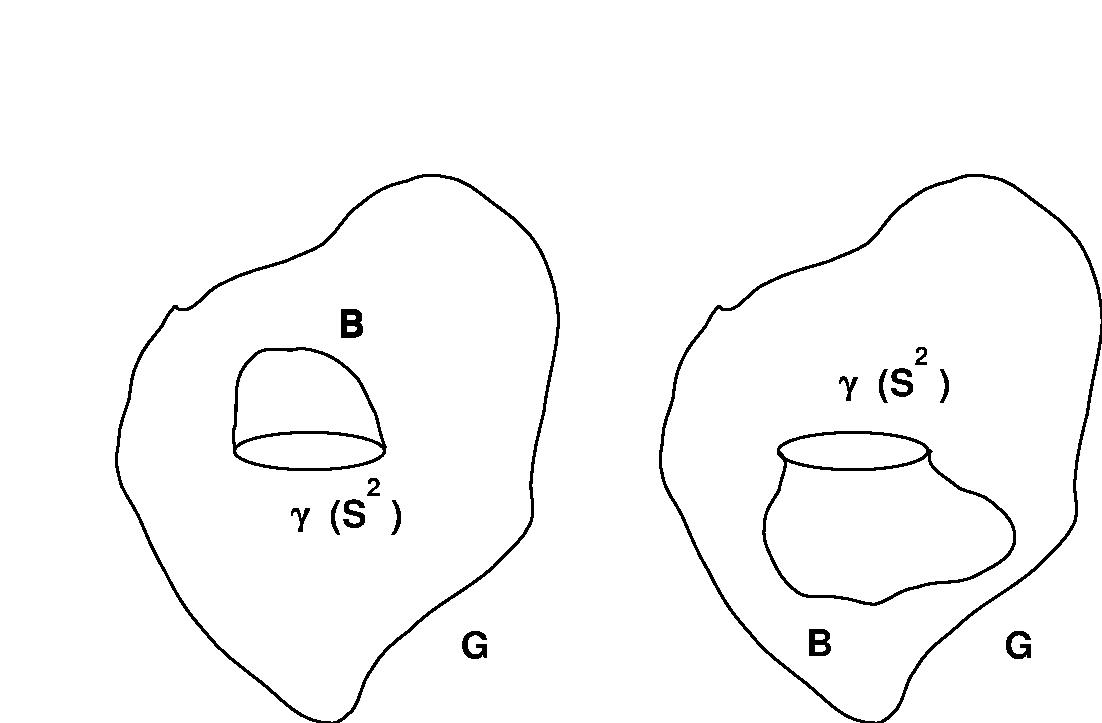
\includegraphics[width=100mm]{fig3}  
  \caption{Два продолжения поля на трехмерное многообразие}
  \label{fig:1}
\end{figure}

Разность значений члена Весса-Зумино $\Delta\Gamma$ на этих многообразиях
дается правой частью уравнения (\ref{eq:73}) с интегралом, продолженным на все компактное трехмерное
пространство. Так как оно топологически эквивалентно три-сфере, получаем
\begin{equation}
  \label{eq:75} \Delta\Gamma= - \frac{i }{24\pi} \int_{S^3}\epsilon_{ijk} Tr'\left( \tilde
g^{-1}\frac{\partial \tilde g}{\partial y^i} \tilde g^{-1}\frac{\partial \tilde g}{\partial y^j}
\tilde g^{-1}\frac{\partial \tilde g}{\partial y^k}\right) d^3y
\end{equation}
$\Delta\Gamma$ определен по модулю $2\pi i$, поэтому Евклидов функциональный интеграл
с весом $exp(-\Gamma)$ хорошо определен. Значит константа связи, умножаемая на этот член, должна
быть целочисленной.

Уравнение движения для полного действия (\ref{eq:4}):
\begin{equation}
  \label{eq:77}
  \partial^{\mu}(g^{-1}\partial_{\mu}g)+\frac{a^2 ik}{4\pi}\epsilon_{\mu\nu}\partial^{\mu}(g^{-1}\partial^{\nu}g)=0
\end{equation}
В комплексных координатах оно записывается в виде
\begin{equation}
  \label{eq:78}
  (1+\frac{a^2 k}{4\pi})\partial_z(g^{-1}\partial_{\bar z}g)+(1-\frac{a^2 k}{4\pi})\partial_{\bar z}(g^{-1}\partial_z g)=0
\end{equation}
Видно, что при $a^2=\frac{4\pi}{k}$ у нас имеются законы сохранения
\begin{equation}
  \label{eq:79}
  \partial_z(g^{-1}\partial{\bar z}g)=0
\end{equation}
Для токов
\begin{equation}
  \label{eq:72}
  J_z=\partial_z g\;g^{-1}, \qquad J_{\bar{z}}=g^{-1}\partial{\bar z}g
\end{equation}

\begin{equation}
  \label{eq:100}
  \partial_{\bar z}J=0,\quad \partial_z \bar J=0
\end{equation}
То есть голоморфная и антиголоморфная части отщепляются, что является указанием на наличие
конформной инвариантности.

Решение классического уравнения движения имеет вид
\begin{equation}
  \label{eq:80}
  g(z,\bar z)=f(z)\bar f(\bar z)
\end{equation}
при произвольных $f(z)$ и $\bar f (\bar z)$.

Сохранение по отдельности токов $J_z,\; J_{\bar z}$ приводит к инвариантности действия при преобразованиях
\begin{equation}
  \label{eq:81}
   g(z,\bar z)\to \Omega(z)g(z,\bar z)\bar \Omega^{-1}(\bar z)
\end{equation}
где $\Omega,\;\bar \Omega \in G$. То есть мы получили локальную $G(z)\times G(\bar z)$-инвариантность.

Для перехода к квантовому случаю мы переопределяем токи
\begin{equation}
  \label{eq:82}
  J(z)\equiv -k \partial_zg g^{-1}\quad \bar J(\bar z)=k g^{-1}\partial_{\bar z}g
\end{equation}
 При инфинитезимальных преобразованиях $\Omega=1+\omega,\; \bar \Omega =1+\bar \omega$ вариация
 $\delta_{\omega}g=\omega g$, а вариация действия
 \begin{equation}
   \label{eq:11}
   \delta S=-\frac{1}{2\pi}\int d^2 x \left(\partial_{\bar z}Tr(\omega(z)J(z))+\partial_z Tr(\bar
     \omega(\bar z)\bar J(\bar z))\right)
 \end{equation}
Заменяем $d^2 x=-\frac{i}{2} dz d\bar z$, интегрируем по частям и переходим к интегралу по контуру, замыкая
контур в разных направлениях для голоморфной и антиголоморфной частей.
Тогда вариация действия
\begin{equation}
  \label{eq:83}
  \delta_{\omega,\bar\omega}S=\frac{i}{4\pi}\oint dz Tr (\omega(z)J(z))-\frac{i}{4\pi}\oint d\bar z Tr(\bar\omega(\bar z)\bar J(\bar z))
\end{equation}
Раскладывая токи
\begin{equation}
  \label{eq:85}
  \begin{aligned}
    J=\sum J^a t^a,\bar J=\sum \bar J^a t^a \\
    \omega=\sum \omega^a t^a\\
  \end{aligned}
\end{equation}
получаем
\begin{equation}
  \label{eq:86}
  \delta_{\omega,\bar \omega}S=-\frac{1}{2\pi i}\oint dz \sum\omega^a J^a+\frac{1}{2\pi i} \oint d\bar z \sum \bar \omega^a \bar J^a
\end{equation}
Мы также получили тождества Уорда $\delta\left< X\right>=\left<(\delta S)X\right>$
\begin{equation}
  \label{eq:87}
  \delta_{\omega,\bar \omega}\left< X \right>=-\frac{1}{2\pi i}\oint dz \sum\omega^a \left< J^a X\right>+
  \frac{1}{2\pi i} \oint d\bar z \sum \bar \omega^a \left< \bar J^a X\right>
\end{equation}
Для токов из явного вида тока и формулы для преобразования $g$ имеем
\begin{equation}
  \label{eq:88}
  \delta_{\omega}J=[\omega,J]-k\partial_z\omega,\quad \delta_{\omega}J^a=\sum i f_{abc}\omega^b J^c-k\partial_z\omega^a
\end{equation}
Если это подставить в тождество Уорда, то получаем операторное разложение для токов, которое имеет
вид 
\begin{equation}
  \label{eq:89}
  J^a(z) J^b(w) \sim \frac{k\delta_{ab}}{(z-w)^2}+\sum i f_{abc}\frac{J^c(w)}{(z-w)}
\end{equation}
Раскладывая токи в ряд, получаем
\begin{equation}
  \label{eq:90}
  \begin{aligned}
    J^a(z)=\sum_{n\in \mathbb Z}z^{n-1}J^a_n\\
    \left[J^a_n,J^b_m\right]=\sum_c i f^{abc}J^c_{n+m}+kn\delta^{ab}\delta_{n+m,0}
  \end{aligned}
\end{equation}
Теперь мы видим, что компоненты токов образуют аффинную алгебру Ли $\hat g$.


Тензор энергии-импульса вводится при помощи конструкции Сугавары как сумма нормально упорядоченных компонент токов
\begin{equation}
  \label{eq:102}
  T(z)=\frac{1}{2(k+h^v)}\sum_a N(J^a J^a)(z)
\end{equation}
Здесь $h^v$ - дуальное число Кокстера. $h^v=\sum_i \alpha_i^v +1=\frac{1}{2}(\Theta,\Theta+2\rho)$,
а нормальное упорядочение вводится следующим образом: 
\begin{equation}
  \label{eq:12}
  N(AB)(w)=\frac{1}{2\pi i}\oint\frac{dz}{z-w}A(z)B(w)
\end{equation}

Тензор энергии-импульса можно разложить на моды $L_n$
\begin{equation}
  \label{eq:91}
  L_n=\frac{1}{2(k+h^v)}\sum_a\sum_m:J^a_m J^a_{n-m}:
\end{equation}
Тогда коммутационные соотношения для мод $L_n$ имеют вид
\begin{equation}
  \label{eq:92}
  \begin{aligned}
    \left[L_n,L_m\right]=(n-m)L_{n+m}+\frac{c}{12}(n^3-n)\delta_{n+m,0}\\
    c=\frac{k\;\mathrm{dim}g}{k+h^v}\\
    \left[L_n,J^a_m\right]=-mJ^a_{n+m}.
  \end{aligned}
\end{equation}

Таким образом, конструкция Сугавары --- это способ вложения алгебры Вирасоро в универсальную обертывающую аффинной алгебры Ли $\hat{g}$

Полная киральная алгебра модели Весса-Зумино-Виттена равна полупрямому произведению $Vir\ltimes \hat g$

Примарными оказываются поля, которые преобразуются ковариантно под действием $G(z)\times G(\bar z)$,
как $g(z,\bar z)$. В терминах операторного разложения это свойство переформулируется следующим
образом:
\begin{equation}
  \label{eq:84}
  \begin{aligned}
    J^a(z)g(w,\bar w)\sim \frac{-t^a g(w,\bar w)}{(z-w)}\\
    \bar J^a(z)g(w,\bar w)\sim \frac{ g(w,\bar w)t^a}{(z-w)}
  \end{aligned}
\end{equation}
Любое поле $\phi_{\lambda,\mu}$, преобразующееся ковариантно по отношению к некоторому
представлению, заданному весом $\lambda$ в голоморфном секторе и весом $\mu$ в антиголоморфном,
является примарным полем WZW-модели.

В модах это свойство записывается в виде
\begin{equation}
  \label{eq:93}
  \begin{aligned}
    & (J_0^a \phi_{\lambda})=-t^a_{\lambda}\phi_{\lambda}\\
    & (J^a_n\phi_{\lambda})=0\quad \mbox{для}\; n>0\\
  \end{aligned}
\end{equation}
Мы можем сопоставить состояние $\left|\phi_{\lambda}\right>$ полю $\phi_{\lambda}$
  \begin{equation}
    \label{eq:94}
    \phi_{\lambda}(0)=\left|\phi_{\lambda}\right>
  \end{equation}
Тогда условия (\ref{eq:93}) для примарных полей дают
\begin{equation}
  \label{eq:95}
  \begin{aligned}
    & J_0^a\left|\phi_{\lambda}\right>=-t^a_{\lambda}\left|\phi_{\lambda}\right>\\
    & J^a_n\left|\phi_{\lambda}\right>=0 \quad \mbox{для}\; n>0 \\
  \end{aligned}
\end{equation}
Все вторичные состояния имеют вид
\begin{equation}
  \label{eq:97}
  J^{a_1}_{-n_1}J^{a_2}_{n_2}\dots\left|\phi_{\lambda}\right>
\end{equation}

Легко видеть, что действие генераторов алгебры Вирасоро на примарные поля имеет вид
\begin{equation}
  \label{eq:96}
  L_0\left|\phi_{\lambda}\right>=\frac{1}{2(k+h^v)}\sum_aJ^a_0J^a_0\left|\phi_{\lambda}\right>=\frac{(\lambda,\lambda+2\rho)}{2(k+h^v)}\left|\phi_{\lambda}\right>
\end{equation}
Здесь использовано явное выражение для собственных значений квадратичного оператора Казимира.

Примарные поля преобразуются  интегрируемыми конечномерными представлениями, а бесконечномерные и
неинтегрируемые поля зануляют корреляционные функции.
В WZW-моделях примарные поля
принадлежат тензорному произведению неприводимых представлений аффинной алгебры, так как есть
голоморфный и антиголоморфный сектора.


\subsection{Конформные вложения и модулярно-инвариантные статсуммы}
\label{sec:modular-invariance}

При изучении конформной теории поля на плоскости или на сфере 
голоморфный и антиголоморфный сектора можно рассматривать независимо. 
Если мы говорим о применении конформной теории для описания поведения струн, то теория должна быть
определена на римановых поверхностях большего рода ($h>0$), чтобы можно было описывать
взаимодействия струн. Считается, что для этого необходимо (и, возможно, достаточно) чтобы теория была определена на торе.

(Нарисовать картинку штанов).

В теории критического поведения конформная инвариантность имеет место только в критической точке,
где голоморфный и антиголоморфный сектора расцеплены. Но вблизи критической точки эти сектора должны
быть связаны, и так как мы предполагаем плавный переход к критической точке в пространстве
параметров, то эта связь должна сохраняться и в критической точке. Физический спектр теории должен
плавно меняться, когда мы покидаем критическую точку, и связь голоморфного и антиголоморфного
сектора вдали от критической точки должна приводить к ограничениям на набор состояний в критической
точке. Этого можно достичь через геометрию, то есть накладывая граничные условия на состояния. Здесь
естественно рассматривать периодические граничные условия, которые эквивалентны рассмотрению теории
на торе.

%% Наложим периодические граничные условия с периодами $\omega_1, \omega_2,\; \tau=\omega_2/\omega_1$. 
%% Мы хотим вычислить статсумму для теории на торе через генераторы алгебры Вирасоро $L_0,\bar L_0$ и
%% выяснить ее зависимость от параметра $\tau$. Пусть пространственное направление соответствует
%% вещественной оси, а временное - мнимой. Пусть $\omega_1$ направлен вдоль вещественной оси. Через $H$
%% обозначим гамильтониан, а через $P$ - общий импульс системы. Тогда оператор трансляции на $a$
%% параллельно периоду $\omega_2$ имеет вид $\exp(-\frac{a}{|\omega_2|}(H \mathrm{Im} \omega_2-i P \mathrm{Re} \omega_2))$. 
%% Если считать, что $a$ - расстояние в решетке, то такой сдвиг переводит нас с одного ряда на другой
%% параллельно периоду $\omega_2$. Если полный период содержит $m$ ячеек решетки ($|\omega_2|=ma$), то
%% статсумма дается следом оператора сдвига в степени $m$:
%% \begin{equation}
%%   \label{eq:6}
%%   Z(\omega_1,\omega_2)=\mathrm{Tr} \exp-\{H \mathrm{Im} \omega_2-iP\mathrm{Re}\omega_2\}
%% \end{equation}
%% Операторы $H,P$ можно выразить через генераторы алгебры Вирасоро если рассмотреть тор как цилиндр
%% конечной длины со склеенными концами. На цилиндре с длиной окружности $L$ гамильтониан
%% $H=(2\pi/L)(L_0+\bar L_0-c/12)$. Константа добавлена, чтобы вакуумная энергия исчезала в пределе
%% $L\to \infty$. Оператор импульса, который генерирует трансляции вокруг окружности, имеет вид
%% $P=(2\pi i/L)(L_0-\bar L_0)$. Так как мы выбрали $\omega_1$ вещественным и равным $L$, статсумму
%% можно записать в виде
%% \begin{equation}
%%   \label{eq:7}
%%   \begin{split}
%%       Z(\tau)=\mathrm{Tr}\exp \pi i \{(\tau-\bar \tau)(L_0+\bar L_0-c/12)+(\tau+\bar \tau)(L_0-\bar
%%       L_0)\}\\
%%       =\mathrm{Tr} \exp 2 \pi i \{\tau(L_0-c/24)-\bar\tau (\bar L_0-c/24)\}\\
%%   \end{split}
%% \end{equation}
%% Или, если ввести $q=\exp 2\pi i \tau$
%% \begin{equation}
%%   \label{eq:2}
%%   Z(\tau)=Tr \left (q^{L_0-c/24}\bar{q}^{\bar{L}_0-c/24}\right)
%% \end{equation}
%% Это выражение, на самом деле --- сумма характеров представлений алгебры Вирасоро (конформных семейств).
%% 
%% Двумерный тор представляет собой фактор пространство $\mathbb{R}^2\approx \mathbb{C}$ по отношениям
%% эквивалентности $z\sim z+w_1$ and $z\sim z+w_2$, где $w_1$ и $w_2$ не параллельны.
%% 
Разные параметризации тора связаны модулярными преобразованиями, таким образом возникает требование
модулярной инвариантности статсуммы.

При помощи конформных преобразований можно перейти к таким координатам, в которых соотношения
эквивалентности для тора (граничные условия) записываются в виде $z\sim z+1$ и $z\sim z+\tau$, где $\tau$ в верхней полуплоскости
$\mathbb{C}$.
%% 
%% Легко видеть, что $\tau$, $T(\tau)=\tau+1$ и $S(\tau)=-\frac{1}{\tau}$ описывают
%% конформно-эквивалентные торы. Отображения $T$ и $S$ порождают группу
%% $SL(2,\mathbb{Z})/\mathbb{Z}_2$, состоящую из матриц вида
%% \begin{equation}
%%   \label{eq:99} A=
%%   \begin{pmatrix} a & b\\ c & d
%%   \end{pmatrix} \quad\mbox{где}\; a,b,c,d\in\mathbb{Z},\quad ad-bc=1,
%% \end{equation}
%% и матрицы $A$ и $-A$ действуют одинаково на $\tau$
%% \begin{equation}
%%   \label{eq:100} \tau\to A\tau=\frac{a\tau+b}{c\tau+d}
%% \end{equation}
%% $\tau$ называется модулярным параметром, а группа $SL(2,\mathbb{Z})/\mathbb{Z}_2$ ---
%% модулярной группой.
%% 
Конформная теория поля задаётся примарными полями $\Phi_a$ с конформными размерностями $\Delta_a$.

Примарные поля живут в пространствах $\mathcal{H}_{(i,j)}$, которые представляют собой тензорные
произведения неприводимого представления $\mathcal{H}_j$ киральной алгебры и неприводимого
представления $\bar{\mathcal{H}}_{\bar{j}}$ антикиральной алгебры. Тогда статсумма на торе
(\ref{eq:2}) может быть записана в виде
\begin{equation}
  \label{eq:9}
    Z(\tau)=\sum_{(j,\bar j)}\chi_j(q)\bar \chi_{\bar j}(\bar q)
\end{equation}
где $\chi_j$ --- нормализованный характер представления $\mathcal{H}_j$,
\begin{equation}
  \label{eq:5} \chi_j(\tau)=Tr_{\mathcal{H}_j}(q^{L_0-\frac{c}{24}})\quad \mbox{где}\; q=e^{2\pi i
\tau}
\end{equation}

Характеры переходят друг в друга при модулярных преобразованиях:
\begin{equation}
  \label{eq:107} \chi_j\left(-\frac{1}{\tau}\right)=\sum_k S_{jk}\chi_k(\tau)\quad \mbox{и}\quad
\chi_j(\tau+1)=\sum_kT_{jk}\chi_k(\tau),
\end{equation}
где $S$ и $T$ --- постоянные матрицы. 

Для WZW-моделей примарные поля определяются старшими весами  $\hat \lambda, \hat \xi$ соответствующих представлений алгебры $\mathfrak{g}$. Тогда
\begin{equation}
  \label{eq:6} \mathcal{H}=\bigoplus_{\hat \lambda,\hat \xi\in P^{(k)}_{+}}M_{\hat \lambda,\hat \xi}
L_{\hat \lambda}\otimes L_{\hat \xi}
\end{equation}

Коэффициенты ветвления для вложения аффинной подалгебры Ли в аффинную алгебру можно использовать для
построения модулярно-инвариантной статсуммы в соответствующей WZW-модели. Когда рассматривается
теория на торе,  набор физически допустимых полей ограничен требованиями модулярной инвариантности.

Простейший модулярный инвариант можно записать следующим образом:
\begin{equation}
  \label{eq:34}
   Z(\tau)=\sum_{ \mu\in P^{+}_{\mathfrak{g}}} \chi_{\mu}(\tau)\bar \chi_{\mu}(\bar \tau)
\end{equation}
Здесь суммирование ведется по всем конформным семействам (то есть по всем представлениям алгебры
$\mathfrak{a}$).

Другие модулярные инварианты в WZW-модели с алгеброй $\mathfrak{a}$ можно получить, если существует
алгебра $\mathfrak{g}$, в которую $\mathfrak{a}$ вкладывается конформно. (Я сейчас поясню, что это
значит). 

Представления алгебры можно рассматривать как сумму представлений подалгебры. 

Если мы рассмотрим редукцию характеров аффинной алгебры
\begin{equation}
  \label{eq:8}
   \pi_{\mathfrak{a}}(ch L^{\mu}_{\mathfrak{g}})=
  \sum_{\nu\in P^{+}_{\mathfrak{a}}}b^{(\mu)}_{\nu} ch L^{\nu}_{\mathfrak{a}}
\end{equation}
и подставим разложение в формулу \eqref{eq:34}, то модулярная инвариантность сохранится. То есть из
диагонального инварианта для алгебры $\mathfrak{g}$ мы получаем новый не диагональный инвариант для
подалгебры $\mathfrak{a}$. Но возникает вопрос, будет ли теория, полученная таким образом, самосогласованной, сохранится ли в
ней конформная инвариантность.

Пусть $J^{a_j}_{-n_j}$ и $\tilde{J}^{a'_j}_{-n_j}$ --- понижающие операторы алгебр  $\mathfrak{g}$ и
$\mathfrak{a}\subset\mathfrak{g}$.  $\pi_{\mathfrak{a}}$ --- проекционный оператор
$\pi_{\mathfrak{a}}:\mathfrak{g}\longrightarrow \mathfrak{a}$. В теории, связанной с  $\mathfrak{g}$
с вакуумом $\left|\lambda\right>$ будут следующие состояния:
\begin{equation}
  \label{eq:109}
  J^{a_1}_{-n_1}J^{a_2}_{-n_2}\dots\left|\lambda\right>\quad n_1\geq n_2\geq \dots>0.
\end{equation}
Вакуум $\mathfrak{g}$-инвариантен, то есть $J_0^a\left|0\right>=0$. При проекции на подалгебру
$\mathfrak{a}$ состояния примут вид
\begin{equation}
  \label{eq:110}
  \tilde{J}^{a'_1}_{-n_1}\tilde{J}^{a'_2}_{-n_2}\dots\left|\pi_{\mathfrak{a}}(\lambda)\right>.
\end{equation}
Из $\mathfrak{g}$-ивариантности вакуума следует его $\mathfrak{a}$-инвариантность, но для тензора
энергии-импульса в общем случае это не так. Поэтому тензор энергии-импульса большей теории должен
состоять только из генераторов $\tilde{J}$. Тогда $T_{\mathfrak{g}}=T_{\mathfrak{a}}\Rightarrow
c(\mathfrak{g})=c(\mathfrak{a})$. Это приводит к уравнению
\begin{equation}
  \label{eq:111}
  \frac{k\;\mathrm{dim}\,\mathfrak{g}}{k+g}=\frac{x_e k\; \mathrm{dim}\,\mathfrak{a}}{x_ek+a}
\end{equation}
Здесь $x_e$ --- индекс вложения, а  $g$, $a$ --- дуальные числа Кокстера, которые характеризуют алгебры.

Можно показать, что только для представлений уровня 1 это равенство удовлетворяется. То есть класс
конформных вложений не слишком широк и существует полная их классификация. Кроме того, для
конформных вложений существуют специальные методы разложения представлений.

Модулярная инвариантность статсуммы для полей, принадлежащих представлениям алгебры  $\mathfrak{g}$,
сохраняется при проекции на подалгебру $\mathfrak{a}$. Если все представления $\mathfrak{g}$ в теории
удовлетворяют описанным требованиям, то при проекции мы получаем конформную теорию поля.

Существует теорема о том, что для конформного вложения  $\mathfrak{a}\subset\mathfrak{g}$ только
конечное число коэффициентов ветвления отлично от нуля. Поэтому после того, как мы разложили все
представления $\mathfrak{g}$ мы подставляем результаты в выражение для статсуммы и получаем
модулярно-инвариантную статсумму для вложенной теории. Такая статсумма уже не будет иметь
диагональный вид:
\begin{equation}
  \label{eq:36}
   Z_{\mathfrak{a}}(\tau)=\sum_{ \nu,\lambda\in P^{+}_{\mathfrak{a}}} \chi_{\nu}(\tau)M_{\nu\lambda}\bar \chi_{\lambda}(\bar \tau)
\end{equation}
Наша работа посвящена разработке общего метода редукции представлений аффинных алгебр Ли, поэтому
случай конформных вложений --- лишь один из примеров применения нашего метода. Однако в этом случае
физический смысл наиболее очевиден. 

Теперь я перейду к краткому объяснению метода и примерам вычислений.

\section{Рекуррентные соотношения для коэффициентов ветвления}
\label{sec:branching}

Ранее для вычисления коэффициентов ветвления был предложен способ, основанный на преобразовании
формулы Вейля-Каца для характеров представлений аффинных алгебр Ли в рекуррентное соотношение для
коэффициентов ветвления. Однако исходный алгоритм не работал для не максимальных вложений. В данной
работе была решена данная проблема и предложено обобщение рекуррентных соотношений. 

Используя формулу Вейля-Каца мы выделяем два набора элементов в весовом пространстве. Первый набор $\Gamma$
называется веером и описывает вложение подалгебры $\mathfrak{a}$ в алгебру $\mathfrak{g}$. Веер
универсален, в том смысле, что он может быть использован для разложения любого из представлений.
Другой набор элементов весового пространства $\Psi ^{\left( \mu \right) }$ называется набором
аномальных весов. Он описывает раскладываемое представление без явного его построения. 

После этого процесс вычисления коэффициентов ветвления можно реализовать при помощи следующей
рекуррентной формулы:
\begin{equation}
  \label{eq:1}
  \begin{array}{c}
      k_{\xi }^{\left( \mu \right) }=-\frac{1}{s\left( \gamma _{0}\right) }\left(
  \sum_{\omega\in W_{\bot}\backslash W} \epsilon(\omega)\; {\rm dim}\left(L^{\pi_{\mathfrak{a}_{\bot}}(\omega(\mu+\rho))-\rho_{\mathfrak{a}_{\bot}}}_{\mathfrak{a}_{\bot}}\right) \delta_{\xi-\gamma_0,\pi_{\mathfrak{a}}(\omega(\mu+\rho)-\rho)}+ \right.\\
\left.
+\sum_{\gamma \in
\Gamma _{\frak{a}\subset \frak{g}}}s\left( \gamma +\gamma _{0}\right) k_{\xi
+\gamma }^{\left( \mu \right) }\right)

  \end{array}
\end{equation}
Здесь $\mathfrak{a}_{\bot}$ --- это подалгебра, ``натянутая'' на корни $\mathfrak{g}$, ортогональные
к корневой системе подалгебры  $\mathfrak{a}$, $W_{\bot}$ --- соответствующая этим корням группа Вейля,
$\Gamma_{\mathfrak{a}\subset \mathfrak{g}}$ --- веер --- набор весов в разложении знаменателя $$\prod_{\alpha\in \Delta^{+}\setminus \Delta^{+}_{\mathfrak{a}_{\bot}}}
(1-e^{-\pi_{\mathfrak{a}}(\alpha)})^{\mathrm{mult}(\alpha)-\mathrm{mult}_{\mathfrak{a}}(\pi_{\mathfrak{a}}(\alpha))}$$, а $s(\gamma)$ ---
коэффициент при  $e^{\gamma}$ в этом разложении.

Набор аномальных весов $\Psi^{(\mu)}$ дает член с $\delta$-символом.

Это рекуррентное соотношение позволяет нам сформулировать следующий алгоритм вычисления
коэффициентов ветвления, который осуществляется без явного построения исходного представления или
представлений, входящих в разложение.
\begin{enumerate}
\item Построить наборы положительных корней $\Delta^{+}$ и $\Delta_{\mathfrak{a}}^{+}$.
\item Выбрать те положительные корни $\alpha\in \Delta^{+}$, которые ортогональны корневому
  подпространству  $\mathfrak{a}$ и собрать их в набор $\Delta^{+}_{\bot}$.
\item Построить множество весов $\Gamma$, которое мы называем ``веером''.
\item Найти множество $\widehat{\Psi^{(\mu)}}=\left\{\omega(\mu+\rho)-\rho;\; \omega\in W\right\}$
  аномальных весов представления $L^{(\mu)}_{\mathfrak{g}}$.
\item Выбрать в нем веса $\left\{ \lambda=\omega(\mu+\rho) | \pi_{\mathfrak{a}_{\bot}}\lambda \in
    \bar{C}_{\mathfrak{a}_{\bot}} \right\}$. Это можно легко сделать, так как у нас есть набор
  $\Delta^{+}_{\bot}$ и мы можем проверить, лежит ли вес $\pi_{\mathfrak{a}_{\bot}}\lambda$ в
  главной камере Вейля алгебры $\mathfrak{a}_{\bot}$. Для этого все скалярные произведения этого
  веса $\lambda$ с корнями из  $\Delta^{+}_{\bot}$ должны быть неотрицательны.
\item Далее для весов $\lambda=\omega(\mu+\rho),\; \pi_{\mathfrak{a}_{\bot}}\lambda\in
  \bar{C}_{\mathfrak{a}_{\bot}}$ мы вычисляем размерность соответствующих представлений
  $\mathrm{dim}\left(L^{\pi_{\mathfrak{a}_{\bot}}(\omega(\mu+\rho))-\rho_{\mathfrak{a}_{\bot}}}_{\mathfrak{a}_{\bot}}\right)$
  при помощи формулы Вейля и набора $\Delta^{+}_{\bot}$.
\item Далее рекуррентно вычисляются аномальные коэффициенты ветвления, а внутри главной камеры Вейля
  алгебры $\mathfrak{a}$ аномальные коэффициенты совпадают с настоящими коэффициентами ветвления.
\end{enumerate}

Сейчас я поясню всю процедуру на примере редукции представления простой алгебры $B_2$ ($so(5)$) на
подалгебру $A_1$ ($so(3)$), а потом расскажу про аффинные алгебры Ли.

\subsection{Примеры}
\label{sec:examples}

Я начну с примера вычисления в случае конечномерных простых алгебр Ли, так как его легко нарисовать.

Рассмотрим регулярное вложение  $A_1$ в $B_2$. Вот на рисунке корневая системы алгебры $B_2=so(5)$.
Корень  $\beta$ вложенной алгебры $A_1$ равен $\alpha_1+2\alpha_2$.

Функция $s(\gamma)$ и веер $\Gamma$ строятся исходя из корневых систем $\mathfrak{g}, \mathfrak{a}$
$\frac{\pi_{\mathfrak{a}}\left(\prod_{\alpha\in \Delta^{+}_{\mathfrak{g}}\setminus
      \Delta^{+}_{\mathfrak{a}}} \left(1-e^{-\alpha}\right) \right)}{\prod_{\beta\in
    \Delta^{+}_{\mathfrak{a}}} \left(1-e^{-\beta}\right) }$ и получается
\begin{equation}
  \label{eq:22}
  (1,2),\; (2,-1)
\end{equation}
Вторая компонента - значение $s(\gamma)$.

Опишем редукцию первого фундаментального представления $B_2$. Старший вес изображен на рисунке.
\begin{figure}[ph]
  \noindent\centering{
    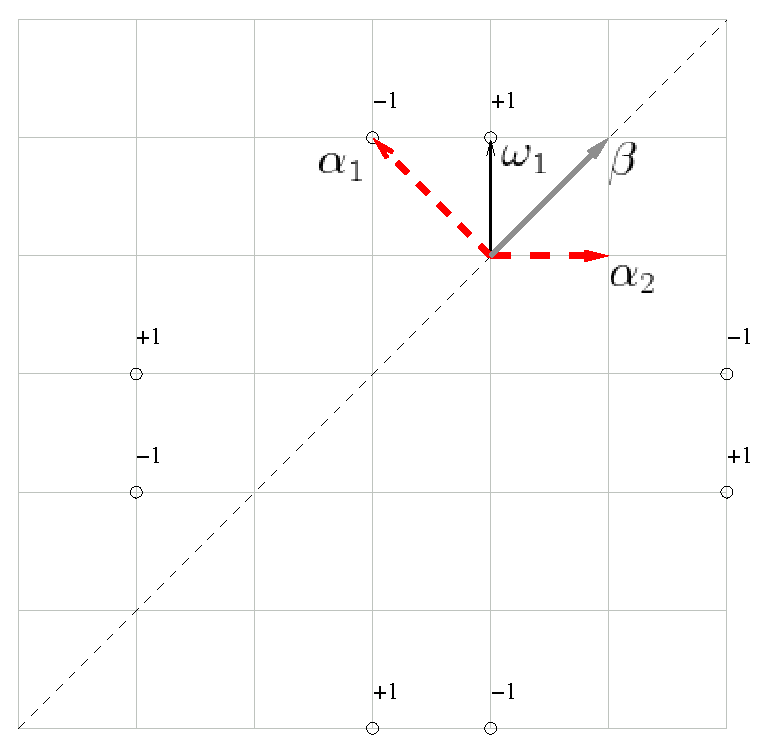
\includegraphics[width=90mm]{B2_A1}
  }
  \caption{Регулярное вложение $A_1$ в $B_2$}
  \label{fig:B2_A1}
\end{figure}
Вот набор аномальных весов $\omega(\mu+\rho)-\rho,\; \omega\in W$ с соответствующими четностями
отражений $\epsilon(\omega)$.
Теперь мы факторизуем группу Вейля $W$ по подгруппе $W_{\bot}=\left\{\omega_1\right\}$. Получаем
следующий набор весов и размерностей представлений  $L^{\pi_{\mathfrak{a}_{\bot}}(\omega(\mu+\rho))-\rho_{\mathfrak{a}_{\bot}}}_{\mathfrak{a}_{\bot}}$:
\begin{figure}[h!tb]
  \noindent\centering{
    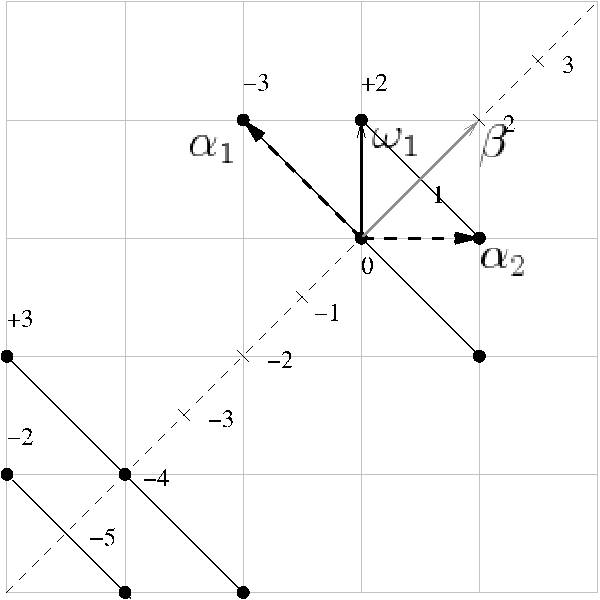
\includegraphics[width=90mm]{B2_A1_2}
  }
  \caption{Аномальные веса и соответствующие $\mathfrak{a}_{\bot}=A_1$-модули}
  \label{fig:B2_A1_2}
\end{figure}

Затем мы проектируем эти веса и размерности на корневое подпространство подалгебры
$\mathfrak{a}=A_1$ и получаем следующие аномальные веса и их кратности:
\begin{equation}
  \label{eq:25}
  (1,2),\; (0,-3),\; (-4,3),\; (-5,-2)
\end{equation}

Аномальный коэффициент ветвления  $k^{(1,0)}_{1}=2$, для коэффициента $k^{(1,0)}_{0}$ из
рекуррентного соотношения получаем
\begin{equation}
  \label{eq:23}
  k^{(1,0)}_{0}=-1\cdot k^{(1,0)}_2 +2\cdot k^{(1,0)}_1 - 3\cdot \delta_{0,0} = 1
\end{equation}

В работе рассмотрено большое число примеров вложений аффинных алгебр Ли. На самом деле мы написали
программу, которая может строить такие примеры автоматически для алгебр Ли не слишком большого
ранга.

Я сейчас покажу результаты применения нашего алгоритма для одного из примеров конформных вложений.

Рассмотрим такое вложение $\mathfrak{a}\subset \mathfrak{g}$, где
$\mathfrak{a}=\hat{A_1}\oplus \hat{A_1}$, а $\mathfrak{g}= \hat{A_3}$. Это
вложение является аффинным расширением специального вложения конечномерных алгебр Ли $A_1\oplus
A_1\subset A3$. ($su(2)\oplus su(2)\subset su(4)$).
\begin{comment}
 Это специальное вложение строится следующим образом: берем четырехмерное
представление $A_1\oplus A_1$ со старшим весом $(1,1)$. Вот веса этого представления
\ref{fig:A_1+A_1_to_A3}, их координаты в базисе фундаментальных весов: $\nu_1=(1,1),\; \nu_2=(-1,1),\; \nu_3=(1,-1),\; \nu_4=(-1,-1)$.

\begin{figure}[h]
  \begin{multicols}{2}
    \hfill
    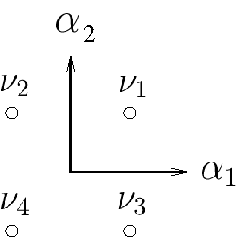
\includegraphics[width=50mm]{A_1+A_1_to_A3}
    \hfill
    \caption{Представление для специального вложения $A_1\oplus A_1\subset A3$}
    \label{fig:A_1+A_1_to_A3}
    \hfill
    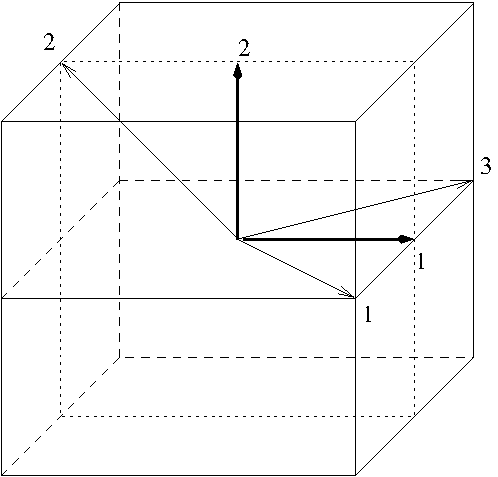
\includegraphics[width=50mm]{A1+A1-A3}
    \hfill
    \caption{Вложенные корни $A_1\oplus A_1\subset A3$}
    \label{fig:A1+A1-A3}
  \end{multicols}
\end{figure}

Тогда матричные элементы представления генераторов подалгебры Картана $b_1,b_2$ в базисе Вейля
даются выражениями
\begin{equation}
  d(b_i)=\mathrm{diag}\left(\frac{2(\nu_1,\alpha_i)}{(\alpha_i,\alpha_i)},\frac{2(\nu_2,\alpha_i)}{(\alpha_i,\alpha_i)},\frac{2(\nu_3,\alpha_i)}{(\alpha_i,\alpha_i)},\frac{2(\nu_4,\alpha_i)}{(\alpha_i,\alpha_i)}\right),
\end{equation}
так что $d(b_1)=\mathrm{diag}(1,-1,1,-1),\;
  d(b_2)=\mathrm{diag}(1,1,-1,-1).$
\end{comment}
Вложенные корни $\alpha_1,\alpha_2$ подалгебры $A_1\oplus A_1$
выражаются через корни $\tilde{\alpha}_i$ алгебры  $A_3$
\begin{equation}
  \label{eq:37}
  \begin{array}{l}
     \alpha_1=\frac{1}{2}(\tilde{\alpha}_1+\tilde{\alpha}_3)\\
     \alpha_2=\frac{1}{2}(\tilde{\alpha}_1+2\tilde{\alpha}_2+\tilde{\alpha}_3)
  \end{array}
\end{equation}
\begin{comment}
Они изображены на рисунке \ref{fig:A1+A1-A3}.
\end{comment}

Вложение имеет индексы  $(2,2)$ и является конформным, так как $c(A_1\oplus A_1)=c(A_1)+c(A_1)=2\frac{x_e \mathrm{dim}(A_1)}{x_e+2}=\frac{\mathrm{dim}A_3}{5}=c(A_3)$.

Для построения модулярно-инвариантной статсуммы нам нужно знать редукцию фундаментальных
представлений $\widehat{su(4)}$. Фундаментальные веса имеют следующие координаты в ортогональном базисе
\begin{equation}
  \begin{array}{lll}
     \omega_0 & = & (0,0,0,0;1;0)\\
     \omega_1 & = & (\frac{3}{4},-\frac{1}{4},-\frac{1}{4},-\frac{1}{4}; 1; 0)\\
     \omega_2 & = & (\frac{1}{2},\frac{1}{2},-\frac{1}{2},-\frac{1}{2}; 1; 0)\\
     \omega_3 & = & (\frac{1}{4},\frac{1}{4},\frac{1}{4},-\frac{3}{4}; 1; 0) \\
  \end{array}
\end{equation}


Множества положительных корней  $\Delta^{+}$ и $\Delta_{\mathfrak{a}}^{+}$:
\begin{equation}
  \label{eq:38}
  \begin{array}{lll}
    \Delta^{+} &=&\left\{\co{\Delta}^{+}=\{\tilde{\alpha}_1, \tilde{\alpha}_2, \tilde{\alpha}_3, \tilde{\alpha}_1+\tilde{\alpha}_2, \tilde{\alpha}_2+\tilde{\alpha}_3, \tilde{\alpha}_1+\tilde{\alpha}_2+\tilde{\alpha}_3\};\right.\\
    &\; & \quad\left.\co{\Delta}+n\delta;\;     +n\delta\;\mbox{с кратностью}\; 3;\; n=1,2,\dots,\right\}\\
    \Delta_{\mathfrak{a}}^{+} &=& \{  \alpha_1,\alpha_2;\;\pm \alpha_1-n\delta,\pm
    \alpha_2-n\delta;\; -n\delta\; \mbox{с кратностью} \; 2;\; n=1,2,\dots\}\\
  \end{array}
\end{equation}

Набор $\Delta^{+}_{\bot}$ пуст.
Веер  $\Gamma _{\frak{a}\subset \frak{g}}$ показан на рисунке \ref{fig:A1+A1-A3_fan}. Конечные координаты
даны в базисе фундаментальных весов $A_1 \oplus A_1$. Элемент $\gamma$ обозначен крестом, если
$s(\gamma)=1$ и кругом, если $s(\gamma)=-1$.
\begin{figure}[h!tb]
  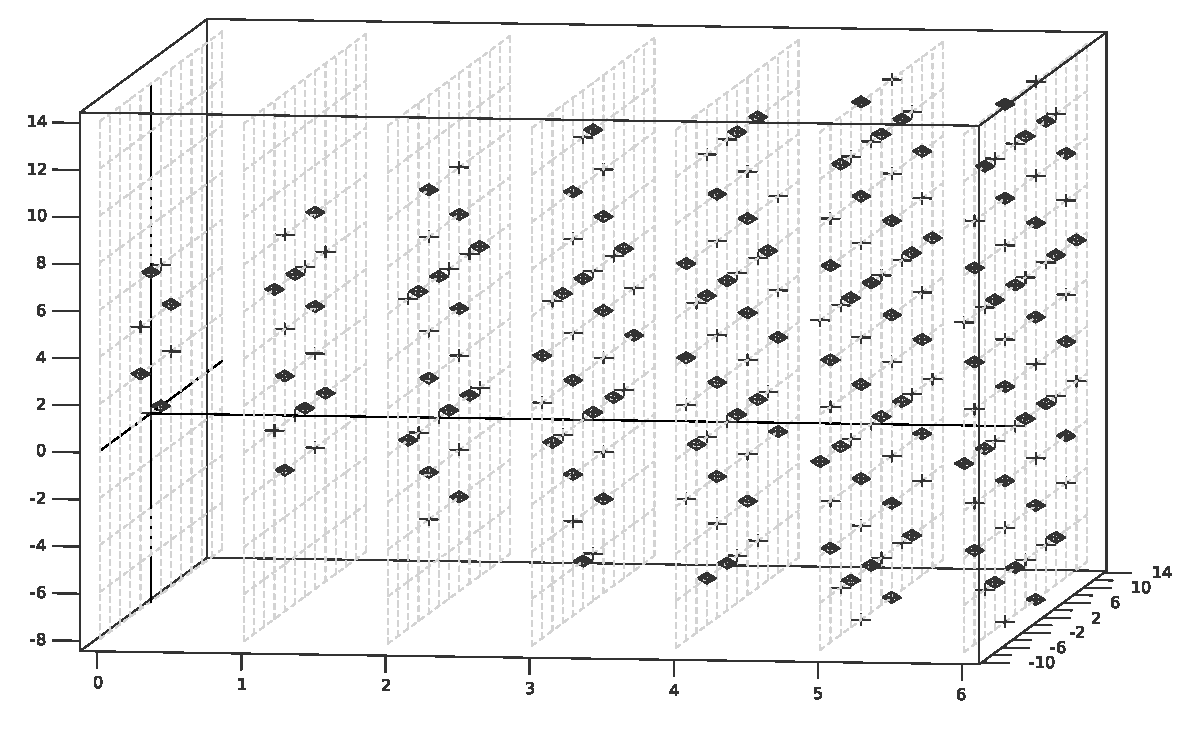
\includegraphics[width=150mm]{A1+A1-A3_fan}
  \caption{Веер для специального вложения $\hat A_1\oplus\hat A_1\subset\hat A_3$}
  \label{fig:A1+A1-A3_fan}
\end{figure}

Мы ограничимся вычислениями до пятого грейда.
\begin{figure}[h!tb]
  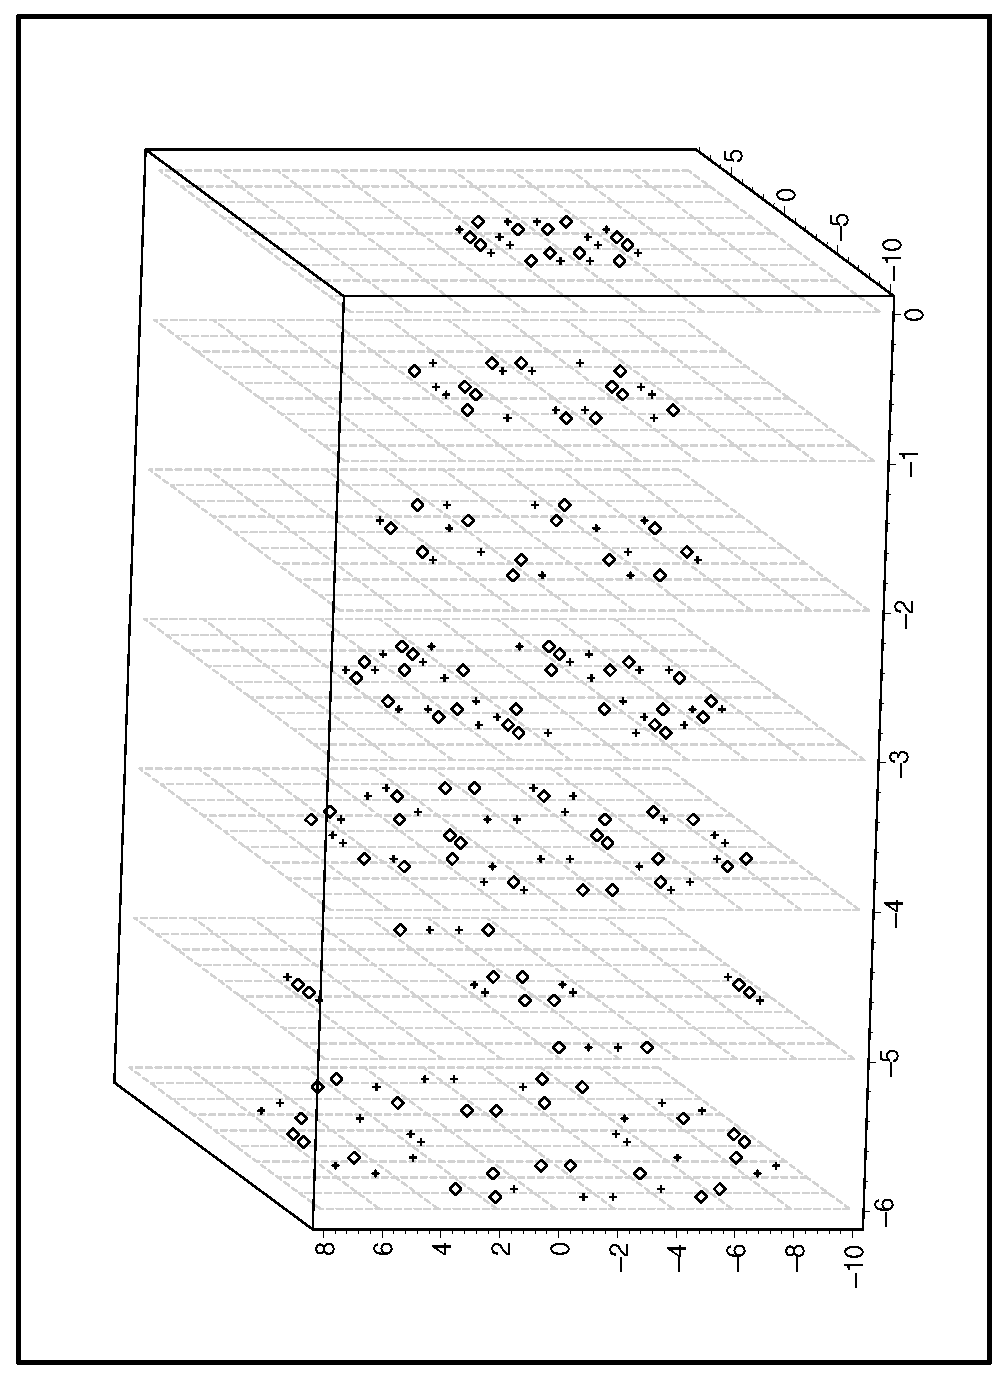
\includegraphics[width=170mm]{A1+A1-A3_anom}
  \caption{Спроектированные аномальные веса $L^{\omega_2}_{A_3}$}
  \label{fig:A1+A1-A3_anom}
\end{figure}

Множество аномальных весов  $\widehat{\Psi^{(\mu)}}=\left\{\omega(\mu+\rho)-\rho;\; \omega\in
  W\right\}$ представления алгебры $\hat{A}_3$ состоит из 192 элементов, их проекции
$\pi_{\mathfrak{a}}\left(\widehat{\Psi^{(\mu)}}\right)$ показаны на рисунке  \ref{fig:A1+A1-A3_anom}
для $\mu=\omega_2=(0,1,0;1;0)$.

Аналогичные картинки для $\omega_0, \omega_1,\omega_3$ я не показываю.

Аномальные коэффициенты ветвления для представления  $L^{(\omega_2)}$ вычислены при помощи
рекуррентных соотношений и показаны на рисунке \ref{fig:A1+A1-A3_branching}. 
\begin{figure}[h!tb]
  \hspace*{-2cm}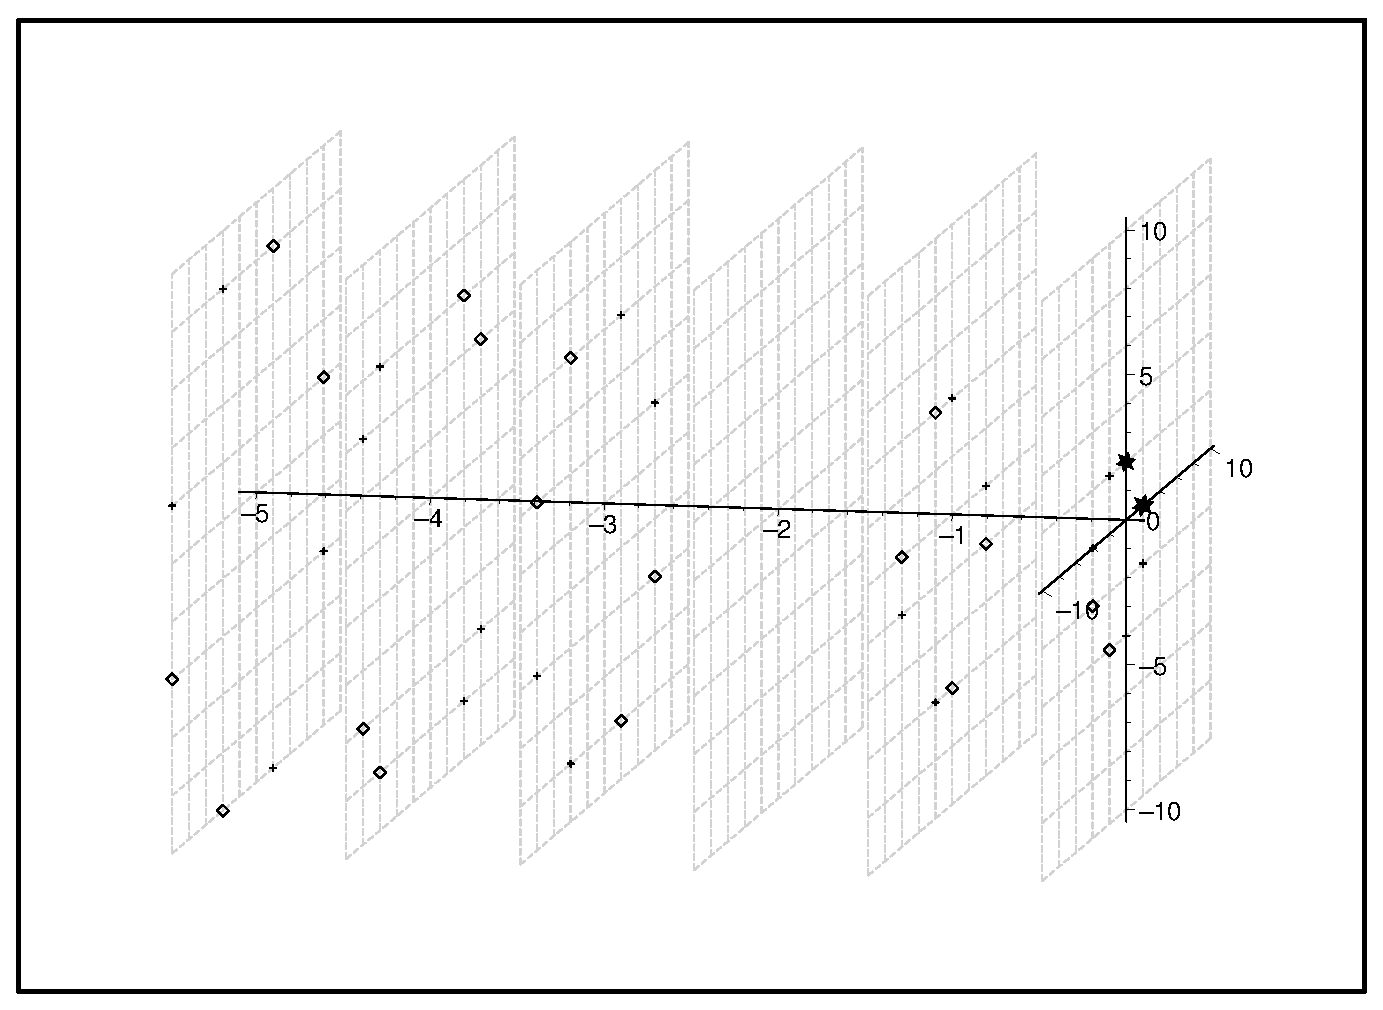
\includegraphics[width=180mm]{A1+A1-A3_branching}
  \caption{Аномальные коэффициенты ветвления для представления $L^{(0,1,0;1;0)}_{A_3}$}
  \label{fig:A1+A1-A3_branching}
\end{figure}

Получаются следующие правила ветвления:
 \begin{equation}
   \label{eq:39}
   \begin{array}{ll}
     L^{(0,0,0;1;0)}_{\hat{A_3}\downarrow \hat{A_1}\oplus \hat{A_1}}= & L_{\hat{A_1}}^{(0;2;0)}\otimes L_{\hat{A_1}}^{(0;2;0)} \\
     L^{(1,0,0;1;0)}_{\hat{A_3}\downarrow \hat{A_1}\oplus \hat{A_1}}= & L_{\hat{A_1}}^{(1;2;0)}\otimes L_{\hat{A_1}}^{(1;2;0)} \\
     L^{(0,1,0;1;0]}_{\hat{A_3}\downarrow \hat{A_1}\oplus \hat{A_1}}= & \left( L_{\hat{A_1}}^{(2;2;0)}\otimes L_{\hat{A_1}}^{(0;2;0)}\right) \oplus \left( L_{\hat{A_1}}^{(0;2;0)}\otimes L_{\hat{A_1}}^{(2;2;0)}\right) \\
     L^{(0,0,1;1;0)}_{\hat{A_3}\downarrow \hat{A_1}\oplus \hat{A_1}}= & L_{\hat{A_1}}^{(1;2;0)}\otimes L_{\hat{A_1}}^{(1;2;0)} \\     
   \end{array}
 \end{equation}

В результате мы получаем модулярно-инвариантную статсумму для WZW-модели с киральной алгеброй $\hat{A}_1\oplus \hat{A}_1$.
\begin{multline}
  \label{eq:40}
  Z=\left|\chi_{(0;2;0)}\chi_{(0;2;0)}\right|^2+2\left|\chi_{(1;2;0)}\chi_{(1;2;0)}\right|^2+ \left|\chi_{(2;2;0)}\chi_{(0;2;0)}+\chi_{(0;2;0)}\chi_{(2;2;0)}\right|^2=\\
  \left|\chi_{(0;2;0)}\right|^4+2\left|\chi_{(1;2;0)}\right|^4+ 4\left|\chi_{(2;2;0)}\chi_{(0;2;0)}\right|^2
\end{multline}

\section{Заключение. Обсуждение перспектив.}
\label{sec:conlusion}

Функции ветвления играют важную роль в coset-моделях. Эти модели строятся путем факторизации
WZW-модели с алгеброй $\mathfrak{g}$ по отношению к модели с подалгеброй $\mathfrak{a}$. Тут функции
ветвления фактически описывают состояния в системе.

Недавно мы заметили, что струнные функции, которые описывают представления, функции ветвления,
описывающие редукцию представлений и функции слияния, которые описывают разложение тензорных
произведений представлений на неприводимые, допускают построение дуальных систем функций. Эти
дуальные функции могут быть построены просто из анализа соответствующих групп и камер Вейля. 
Задача явного построения струнных функций или функций ветвления тогда сведется к обращению матрицы.
Явный вид функций ветвления полезен при изучении coset-моделей. Кроме того, многие
известные результаты могут быть перенесены на дуальные функции, например, результаты Каца о модулярных свойствах
струнных функций и функций ветвления.
В настоящее время мы начали исследовать эти системы дуальных функций. 

Среди других возможных приложений полученных методов можно отметить также приложения в интегрируемых
цепочках, а также в приложения дуальных функций теории модулярных форм. 





\section{Coset-модели}
\label{sec:coset-models}
Ветвления. Функции ветвления и статсуммы. 
Калибровочные WZW-модели. 

\section{SLE}
\label{sec:sle}
SLE на WZW-моделях. Граничные условия. Парафермионы. SLE на coset-моделях.


\begin{abstract}
  Schramm-Loewner evolution appears naturally as the scaling limit of interfaces in lattice models at critical point. Critical behavior of these models can be described by minimal models of conformal field theory.

  We generalize Schramm-Loewner evolution with additional Brownian motion on Lie group to the case of direct product of two groups. We then study connection between SLE description of critical behavior with coset models of conformal field theory. In order to be consistent such construction should give minimal models for certain choice of groups. 

%%    SLE with additional Brownian motion on Lie group $G$ was proposed as generalization to WZNW models of CFT. Martingale property of SLE observables is related to Virasoro null vector conditions for CFT fields and KZ-equations for correlation functions. 
%%  
%%    Minimal models can be obtained from WZNW models by coset construction. Then it is natural to study SLE with additional Brownian motion on coset space $G/H$. We discuss algebraic properties of coset fields and correlation functions which correspond to SLE observables. 
\end{abstract}

\section{Introduction}
Schramm-Loewner evolution, introduced by Oded Schramm in papers \cite{schramm2000scaling} is 

The connection of SLE with CFT was studied in papers \cite{bauer2004conformal,bauer2004cfts,bauer2003sle,bauer2002sle}.

Reviews \cite{rohde2005basic}, \cite{bauer20062d}, \cite{Cardy:2005kh}. 

SLE and conformal field theories with additional symmetries \cite{alekseev2010sle}, \cite{santachiara2008sle,picco2008numerical}, \cite{bettelheim2005stochastic}, \cite{Rasmussen:2004xr}.

\subsection{Schramm-Loewner evolution}
To remind of Schramm-Loewner evolution we first describe simple example.

Consider Ising model on triangular lattice on upper half plane (see Fig. \ref{fig:sle}). We impose following boundary condition: all spins are down on one half of the boundary and all spins are up on another half. Then in any configuration we get an interface delimiting two clusters and connecting zero and infinity. 

\begin{figure}[h]
  \centering{
    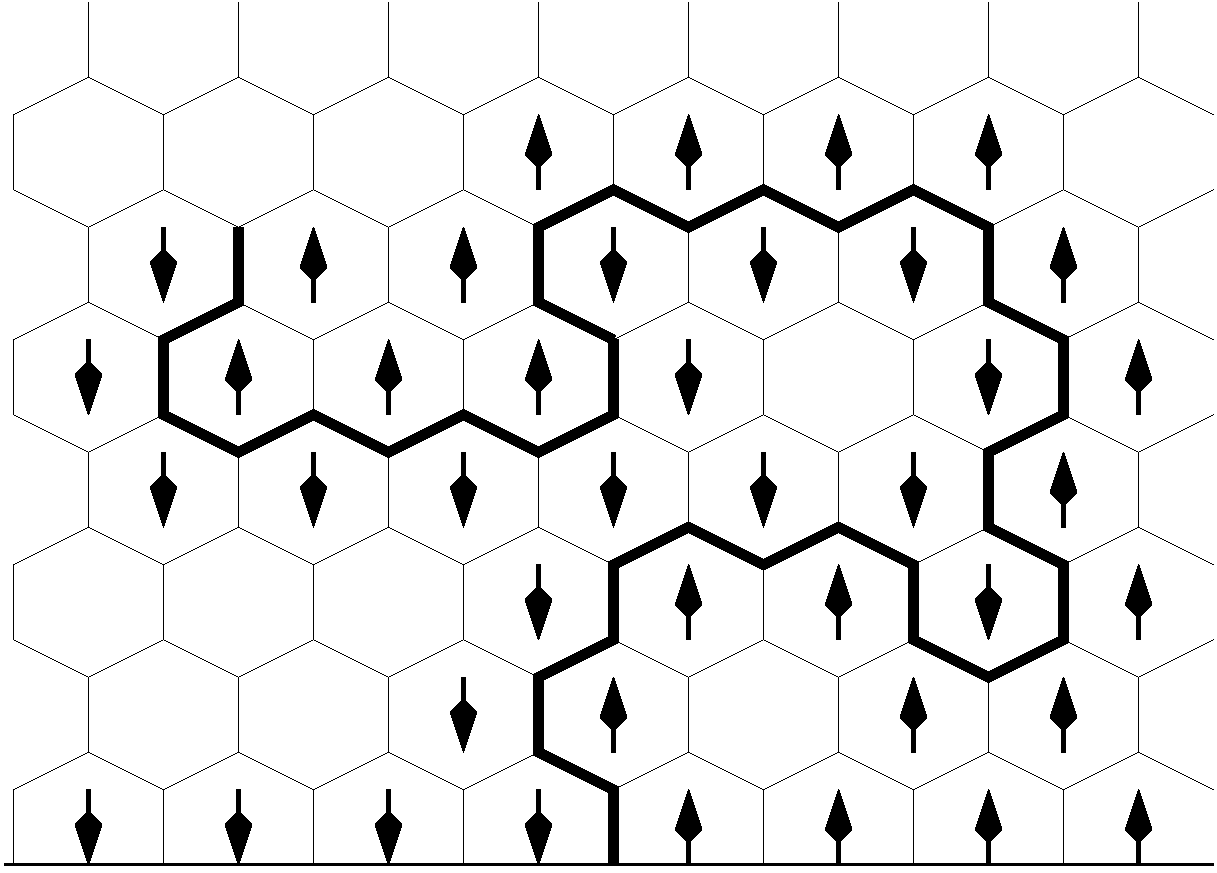
\includegraphics[height=25mm]{explore}
    \caption{SLE -- continuous limit of interfaces}}
  \label{fig:sle}
\end{figure}

Next we consider continuous limit of lattice model. Interface in random configuration of the model tends to random curve. We can think of this curve as of trace of stochastic process which satisfy some stochastic equation. 

In papers [Smirnov, Schramm ... ] it was shown that this equation is
\begin{equation*}
  \frac{\partial g_t(z)}{\partial t} = \frac{ 2}{g_t(z)-\sqrt{\kappa}\xi_{t}} \quad \text{or} \quad       d w _{t}= \frac{2dt}{w_{t} }-\sqrt{\kappa}\xi_{t}
\end{equation*}
The stochastic process which satisfy this equation is called     {\it Schramm-Loewner evolution} on the upper half-plane $\mathbb{H}$.

Here $g_{t}(z)$ is a conformal map from $\mathbb{H}_{t}=\mathbb{H}\setminus \gamma_{t}$ to $\mathbb{H}$ (see Fig. \ref{fig:sle2}).
\begin{figure}[h]
  \centering{
    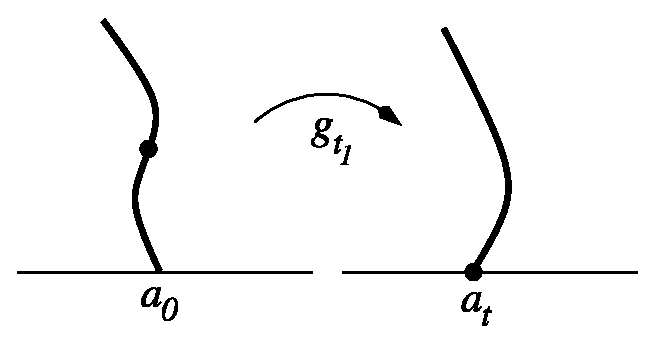
\includegraphics[width=50mm]{loewner}
    \caption{Conformal map}}
  \label{fig:sle2}
\end{figure}

Schramm-Loewner evolution provides conformally-invariant probability measure on trajectories $\gamma_{t}$ in $\mathbb{H}$.

\subsection{Correspondence between SLE and minimal models of CFT}

Now we can look at the observables in the presence of SLE trace. Expectation value of lattice observable on upper half-plane can be calculated as the sum of expectation values of this observable in presence of SLE trace up to some time $t$ multiplied by the probability of this trajectory. 

Consider lattice observable $\mathcal{O}$, then it expectation value can be calculated as
\begin{equation*}
  \prec \mathcal{O} \succ_{\mathbb{H}}=\mathbb{E}\left[\prec\mathcal{O}\succ_{\gamma_{t}}\right]=\sum_{\gamma_{t}} P\left[C_{\gamma_{t}}\right] \prec \mathcal{O} \succ_{\gamma_{t}}
\end{equation*}
Since lattice observable  $\prec \mathcal{O} \succ_{\mathbb{H}}$ does not depend on $t$, hence $\prec\mathcal{O}\succ_{\gamma_{t}}$ is a martingale.

In continuous limit lattice observable tends to CFT correlation function. Since we consider the theory with the boundary, CFT correlation function has following form:
\begin{equation*}
  \prec \mathcal{O} \succ_{\mathbb{H}_{t}}\to \mathcal{F}(\left\{z_{i}\right\})_{\mathbb{H}_{t}}=
  \frac{\left< \mathcal{O}(\{z_{i}\})\phi(z_{t})\phi^{\dagger}(\infty)\right>_{\mathbb{H}_{t}}}{\left<\phi(z_{t})\phi^{\dagger}(\infty)\right>_{\mathbb{H}_{t}}}=
  \frac{\left< ^{g_{t}}\mathcal{O}\phi(\xi_{t})\phi^{\dagger}(\infty)\right>_{\mathbb{H}}}{\left<\phi(z_{t})\phi^{\dagger}(\infty)\right>_{\mathbb{H}}}
\end{equation*}
We assume that $\mathcal{F}$ contains some set of primary fields $\phi_{\lambda_{i}}$ with conformal weights $\lambda_{i}$. Also we have boundary condition changing operators  $\phi$ at the tip of SLE trace and in the infinity.  We can use conformal map  $w(z):\mathbb{H}\setminus\gamma_{t}\to \mathbb{H}$ to rewrite this expression in upper half plane:

\begin{equation}
  \mathcal{F}(\left\{z_{i}\right\})_{\mathbb{H}_{t}}=\prod \left(\frac{\partial w(z_{i})}{\partial z_{i}}\right)^{h_{\lambda_i}} 
  \prod \left(\frac{\partial \bar w(\bar z_{i})}{\partial \bar z_{i}}\right)^{h_{\lambda^{*}_i}}
  \mathcal{F}(\left\{w_{i}, \bar w_{i}\right\})_{\mathbb{H}}
  \label{eq:1}
\end{equation}

Now we want to consider evolution of SLE trace $\gamma_{t}$ from  $t$ to $t+ dt$. First factor in right-hand-side of equation (\ref{eq:1}) gives us
\begin{equation*}
  -\frac{2h_{\lambda_{i}}}{w_{i}^{2}}\left(\frac{\partial w_{i}}{\partial z_{i}}\right)^{h_{\lambda_{i}}}.
\end{equation*}
For transformation of primary fields $\phi_{\lambda_{i}}$ we have 
\begin{equation}
  \label{eq:2}
  d\phi_{\lambda_{i}}(w_{i}) = \mathcal{G}_{i}\phi_{\lambda_{i}}(w_{i})=\left(\frac{2dt}{w_{i}}-\sqrt{\kappa} d\xi_{t}\right) \partial_{w_{i}}\phi_{\lambda_{i}}(w_{i}) 
\end{equation}
We denote generator of this transform by $\mathcal{G}_{i}$.



Continuous limit in critical point leads to CFT correlation function

Now for expectation value of martingale we have this expression.
\begin{equation*}
  \mathbb{E}\left[\prec\mathcal{O}\succ_{\gamma_{t}}\right]=    \mathbb{E}\left[\prec\mathcal{O}\succ_{\gamma_{t+dt}}\right], \quad \mathbb{E}\left[d \prec\mathcal{O}\succ_{\gamma_{t}}\right]=0
\end{equation*}

Now we use Ito calculus to calculate increment of our correlation function. It should be zero so we get the equation:
\begin{equation}
  \left(\prod_{i=1}^{2N}\left(\frac{\partial w_{i}}{\partial z_{i}}\right)^{-h_{i}}\right)\mathbb{E}\left[d 
    \mathcal{F}_{\mathbb{H}_{t}}\right]=\left(-\sum_{i=1}^{2N}\frac{2h_{i}dt}{w_{i}^{2}}+\mathbb{E}\left[\sum_{i=1}^{2N}\mathcal{G}_{i}+\frac{1}{2}
      \sum_{i,j}\mathcal{G}_{i}\mathcal{G}_{j}\right]\right)\mathcal{F}_{\mathbb{H}}
\label{eq:8}
\end{equation}
Then use explicit form of conformal map and obtain
\begin{equation*}
  \left( \sum_{i}\left[-\frac{2h_{i}}{w_{i}^{2}} +\frac{2}{w_{i}}\partial_{w_{i}}\right]+\frac{\kappa}{2}\sum_{i,j}\partial_{w_{i}} \partial_{w_{j}}\right)\mathcal{F}(\left\{z_{i}\right\})=0
\end{equation*}

We can rewrite it as the necessary condition on b.c.c. operator $\phi$:
\begin{equation*}
  (L_{-2}-\frac{\kappa}{2}L_{-1}^{2})\phi=0 \Longrightarrow \phi \left|0\right>  \text{has level 2 null state}, \phi\sim \phi_{1,2} \;\text{or}\; \phi_{2,1}
\end{equation*}
We can see that it can be rewritten as the action of Virasoro generators. Since we have arbitrary observable, this equation is equivalent to the requirement for boundary condition changing operator to have level two null state. 
In case of minimal model we can see that boundary condition chaining operator is primary field $\phi_{1,2}$ or $\phi_{2,1}$.

\section{SLE and WZNW models}
\label{sec:sle-wzw-models}
Now we want to generalize this analysis to rational conformal field theories. First we consider Wess-Zumino-Novikov-Witten model.
\subsection{WZNW models}

 The action for this model can be written in terms of map $g:\mathbb{C}\cup \{\infty\}\sim S^{2}\to G$ from complex plane with infinity or two-sphere to some Lie group $G$:
\begin{multline}
  S=-\frac{k}{8\pi}\int d^2x\; \mathcal{K} (g^{-1}\partial^{\mu}g, g^{-1} \partial_{\mu}g)  
  \\
  - \frac{k }{24\pi^{2}} \int_{B}\epsilon_{ijk} \mathcal{K}\left(
    \tilde g^{-1}\frac{\partial \tilde g}{\partial y^i},\left[
      \tilde g^{-1}\frac{\partial \tilde g}{\partial y^j}
      \tilde g^{-1}\frac{\partial \tilde g}{\partial y^k}\right]\right) d^3y
\end{multline}
The first term is just non-linear sigma-model.

 Here $\mathcal{K}$ is Killing form on Lie algebra $\gf$ of Lie group $G$. The second term is written in terms of continuation from two-sphere $S^{2}$ to three-dimensional manifold $B$ which has two-sphere as the boundary. Since this continuation is non-unique we get the requirement for $k$ to be integer. 

Currents of this model have following form:
  \begin{eqnarray}
    J(z)= -k \partial_zg g^{-1}
    \bar J(\bar z)=k g^{-1}\partial_{\bar z}g
  \end{eqnarray}

Model possess gauge invariance under gauge transformations:
  \begin{equation*}
    g(z,\bar z)\to \Omega(z)g(z,\bar z)\bar \Omega^{-1}(\bar z),
  \end{equation*}
  where $\Omega,\;\bar \Omega \in G$.
Here $\Omega$ and $\bar \Omega$ are independent. 

If we consider infinitesimal gauge transformation $\Omega=1+\omega$ we get Ward identities:
  \begin{equation}
    \label{eq:87}
    \delta_{\omega,\bar \omega}\left< X \right>=-\frac{1}{2\pi i}\oint dz \sum\omega^a \left< J^a X\right>+
    \frac{1}{2\pi i} \oint d\bar z \sum \bar \omega^a \left< \bar J^a X\right>
  \end{equation}

 Then we can get operator product expansion for currents. 
 \begin{equation}
   \label{eq:3}
   <J\phi>\sim \dots
 \end{equation}

If we expand currents to modes
\begin{equation*}
  J^a(z)=\sum\limits_{n\in \mathbb Z}z^{n-1}J^a_n 
\end{equation*}
and use operator product expansion \eqref{eq:3} we get commutation relations of affine Lie algebra $\gfh$:
\begin{equation}
  \left[J^a_n,J^b_m\right]=\sum_c i f^{abc}J^c_{n+m}+kn\delta^{ab}\delta_{n+m,0} 
\end{equation}

This model has conformal invariance which can be seen from 
Sugawara construction. This is way to embed Virasoro algebra into the universal enveloping algebra of affine Lie algebra $\gfh$ ($Vir\subset U(\gfh)$):
\begin{equation}
  \label{eq:4}
  L_n=\frac{1}{2(k+h^v)}\sum\limits_a\sum\limits_m:J^a_m J^a_{n-m}:
\end{equation}
  
Full chiral algebra of the model is semidirect product of affine and Virasoro algebra $\gfh \ltimes Vir$. 

Its commutation relations are
  \begin{equation}
    \label{eq:92}
    \begin{aligned}
      \left[L_n,L_m\right]=(n-m)L_{n+m}+\frac{c}{12}(n^3-n)\delta_{n+m,0}\\
      \left[L_n,J^a_m\right]=-mJ^a_{n+m}
    \end{aligned}
  \end{equation}

Primary fields  $\phi_{\lambda}$ are labeled by highest weights of affine Lie algebra representations. Here we see how Virasoro and affine Lie algebra generators act on primary fields:
  \begin{equation*}
    \begin{aligned}
      & J_0^a\left|\phi_{\lambda}\right>=-t^a_{\lambda}\left|\phi_{\lambda}\right>  \quad    J^a_n\left|\phi_{\lambda}\right>=0 \quad \mbox{for}\; n>0 \\
      & L_0\left|\phi_{\lambda}\right>=\frac{1}{2(k+h^v)}\sum_aJ^a_0J^a_0\left|\phi_{\lambda}\right>=\frac{(\lambda,\lambda+2\rho)}{2(k+h^v)}\left|\phi_{\lambda}\right>=h_{\lambda} \left|\phi_{\lambda}\right>
    \end{aligned}
  \end{equation*}


\subsection{SLE and WZNW models}
Now we want to study Schramm-Loewner evolution in WZNW-models.

Similarly to minimal models we consider observable
\begin{equation*}
  \mathcal{F}(\left\{z_{i}\right\})_{\mathbb{H}_{t}}=
  \frac{\left<\phi_{\Lambda}(z_{t}) \phi_{\lambda_1}(z_{1}) \dots \phi_{\lambda_n}(z_{n}) \phi_{\lambda^{*}_1}(\bar z_{1}) \dots \phi_{\lambda^{*}_n}(\bar z_{n})
      \phi_{\Lambda^{*}}(\infty)\right>}{\left<\phi_{\Lambda}(z_{t})\phi_{\Lambda^{*}}(\infty)\right>}
\end{equation*}
Again we can use conformal map  $w(z):\mathbb{H}\setminus\gamma_{t}\to \mathbb{H}$ to rewrite it on the whole upper half-plane. 
\begin{equation*}
  \mathcal{F}(\left\{z_{i}\right\})_{\mathbb{H}_{t}}=\prod \left(\frac{\partial w(z_{i})}{\partial z_{i}}\right)^{h_{\lambda_i}} 
  \prod \left(\frac{\partial \bar w(\bar z_{i})}{\partial \bar z_{i}}\right)^{h_{\lambda^{*}_i}}
  \mathcal{F}(\left\{w_{i}, \bar w_{i}\right\})_{\mathbb{H}}
\end{equation*}

Consider evolution from $t$ to $t+dt$.
First factor gives us $-\frac{2h_{\lambda_{i}}}{w_{i}^{2}}\left(\frac{\partial w_{i}}{\partial z_{i}}\right)^{h_{\lambda_{i}}}$.

 For fields we have
\begin{equation*}
  d\phi_{\lambda_{i}}(w_{i}) = \mathcal{G}_{i}\phi_{\lambda_{i}}(w_{i})
\end{equation*}
When we consider fields we need to add random gauge transformation (random motion in $G$) to stochastic evolution \cite{bettelheim2005stochastic}, \cite{alekseev2010sle}:
\begin{equation*}
  \mathcal{G}_{i}=\left(\frac{2dt}{w_{i}}-\sqrt{\kappa} d\xi_{t}\right) \partial_{w_{i}}+\frac{\sqrt{\tau}}{w_{i}}\sum_{a=1}^{\mathrm{dim} \gf}\left(d \theta ^{a} t^{a}_{i}\right)
\end{equation*}
Since we have boundary we are working with boundary CFT so we have only half of gauge transformations due to Cardy conditions.

\subsection{SLE martingales in WZNW models}
We use Ito calculus to get the equation from martingale condition:
\begin{equation*}
  \left(-2 \mathcal{L}_{-2}+\frac{1}{2}\kappa \mathcal{L}_{-1}^{2}+\frac{1}{2}\tau\sum_{a} \mathcal{J}^{a}_{-1} \mathcal{J}^{a}_{-1}\right)        \mathcal{F}(\left\{w_{i}, \bar w_{i}\right\})_{\mathbb{H}}=0
\end{equation*}
\begin{equation*}
  \mathcal{L}_{-n}=\sum_{i}\left(\frac{(n-1)h_{\lambda_{i}}}{(w_{i}-z)^{n}}-\frac{1}{(w_{i}-z)^{n-1}}\partial_{w_{i}}\right);\quad \mathcal{J}^{a}_{{-n}}=-\sum_{i}\frac{t^{a}_{i}}{(w_{i}-z)^{n}}
\end{equation*}
Again we can rewrite it as algebraic requirement for  field  which 
correspond to boundary condition changing operator.
\begin{equation*}
  \left| \psi\right>=\left(-2 L_{-2}+\frac{1}{2}\kappa L_{-1}^{2}+\frac{1}{2}\tau\sum_{a} J^{a}_{-1} J^{a}_{-1}\right) \left|\phi_{\Lambda}\right>    
\end{equation*}
is level two null state and if we act on this state with raising operators we should get zero.
\begin{equation*}
  J^{a}_{1} \left|\psi\right>=0, J^{a}_{2}\left|\psi\right>=0.
\end{equation*}
 We use commutation relations and get equations which connects parameters of random motion with level of affine Lie algebra representation. 

We can see that $\kappa+\tau h^{v}=4$ and it is possible to derive additional relations connecting $\kappa, \tau, k$:
\begin{equation*}
  \kappa=\frac{2(h^{v}-2k)}{2h_{\Lambda}h^{v}-k},\quad \tau=\frac{8 h_{\Lambda}-2}{2h_{\Lambda}h^{v}-k}  \quad\text{for}\; k\neq 2h_{\Lambda}h^{v}
\end{equation*}
 Also we get some constraints on possible boundary condition changing operators. 
To get complete classification use Knizhnik-Zamolodchikov equations.


\section{Coset models}
\label{sec:coset-models}
Now we want to generalize analysis of correspondence between SLE and CFT even further and study coset models of conformal field theory.


\subsection{Gauged WZNW-models and coset construction}

Coset models can be realized as gauged Wess-Zumino-Novikov-Witten models. We add gauge fields  $A, \bar{A}$ taking values in Lie algebra $\af\subset \gf$ to the action:
\begin{multline*}
  S(g,A)=S_{WZNW}(g)+\\
  \frac{k}{4\pi}\int d^{2}z \left(\mathcal{K}(A, g^{-1}\bar \partial g)-\mathcal{K}(\bar A, (\partial g ) g^{-1})+\mathcal{K}(A,g^{-1}\bar A g)-\mathcal{K}(A,\bar A)\right)
\end{multline*}
Now current is
\begin{equation*}
  J_{(\gf,\af)}=-k\partial g g^{-1} -k g A g^{-1}
\end{equation*}

From Ward identities we get following expression for the product of gauge field and primary fields:
\begin{equation*}
  \left< A^{b}(z)\phi_{1}\dots \phi_{N}\right>=\frac{2}{k+2 h^{v}_{\af}}\sum_{k}\frac{\tilde{t}^{b}_{k}}{z-z_{k}}\left<\phi_{1}\dots \phi_{N}\right>
\end{equation*}
Here $h_{\af}^{v}$ is the dual Coxeter number of Lie algebra $\af$.

Remember that for WZNW current we have OPE $J_{\gf}^{a}(z)\phi_{i}(w)\sim \frac{-t^{a}_{i}\phi(w)}{z-w}$,  so we see that algebraic structure is connected with the pair of algebras $\gf$ and $\af$, such that $\afh\subset\gfh$. 

Virasoro generators are given by difference of Sugawara expressions:
\begin{equation*}
  L_{n}=L_{n}^{\gf}-L_{n}^{\af}
\end{equation*}

\subsection{Primary fields}
\label{sec:primary-fields}
Primary fields are labeled by pairs of weights $(\mu,\nu)\in \hf_{\gfh}\oplus \hf_{\afh}$  of algebra and subalgebra, such that branching functions $b^{\mu}_{\nu}(q)\neq 0$. But some pairs are equivalent. This equivalence is given by the action of simple currents $(J,\tilde{J})$ such that their conformal weights are equal:  $h_{J}-h_{\tilde{J}}=0$. 

Conformal weight of primary field is equal to
\begin{multline}
  L_0\left|\phi_{(\mu,\nu)}\right>=\left(\frac{1}{2(k+h^v)}\sum_aJ^a_0J^a_0-\frac{1}{2(k+h_{\af}^v)}\sum_b \tilde{J}^b_0 \tilde{J}^b_0 \right)
  \left|\phi_{\lambda}\right>=\\
  \left(\frac{(\mu,\mu+2\rho)}{2(k+h^v)}-\frac{(\nu,\nu+2\rho_{\af})}{2(k+h^v)}\right)\left|\phi_{(\mu,\nu)}\right>
\end{multline}

%% So $G/A$-coset theory is related to $\gf\oplus \bar{\af}$-theory.

It is possible to obtain analogues of KZ-equations:
\begin{equation*}
  \left\{\frac{1}{2}\partial_{i} + \sum_{i\neq j}^{N}\left(\frac{t^{a}_{i}t^{a}_{j}}{k+h^{v}}-\frac{\tilde t^{b}_{i}\tilde t^{b}_{j}}{k+h^{v}_{\af}}\right)\frac{1}{z_{i}-z_{j}}\right\} \left<\phi_{1}(z_{1})\dots \phi_{N}(z_{N})\right>=0
\end{equation*}

\subsection{SLE on coset space}
Consider Lie (semi-)simple group $G$ with Lie algebra $\gf$ and (semi-)simple subgroup $A\subset G$ with Lie algebra $\af\subset \gf$. 
The simplest way to study SLE on $G/A$ coset space is to restrict random walk on group manifold to the coset space by the choice of basis in $\gf$. Assume that generators $\{J^{a};\; a=1\dots \mathrm{dim}\gf\}$ are chosen in such way that $\mathcal{K}(J^{a},J^{b})=h^{\vee}\delta_{ab}$ and $\{J^{a};\; a=\mathrm{dim}\gf-\mathrm{dim}\af\dots \mathrm{dim}\gf\}$ are the generators of subalgebra $\af\subset \gf$. Now we can consider $\mathrm{dim}\gf-\mathrm{dim}\af$-dimensional Brownian motion with generators $d\theta^{a}$ such that $\mathbb{E}(d\theta^{a} \; d\theta^{b})=\delta_{ab};\; a,b=1,\dots,\mathrm{dim}\gf-\mathrm{dim}\af$.

Then for generator of field transformation we can write 
\begin{equation}
  \mathcal{G}_{i}=\left(\frac{2dt}{w_{i}}-\sqrt{\kappa} d\xi_{t}\right) \partial_{w_{i}}+\frac{\sqrt{\tau}}{w_{i}}\left(\sum_{a=1}^{\mathrm{dim}\gf-\mathrm{dim}\af}\left(d \theta ^{a} t^{a}_{i}\right)\right)
\label{eq:5}
\end{equation}
Substituting to equation \eqref{eq:8} we get martingale condition

\begin{equation}
  \left(-2 \mathcal{L}_{-2}+\frac{1}{2}\kappa \mathcal{L}_{-1}^{2}+\frac{\tau}{2}\left( \sum_{a=1}^{\mathrm{dim}\gf-\mathrm{dim}\af} \mathcal{J}^{a}_{-1} \mathcal{J}^{a}_{-1}\right)\right)        \mathcal{F}_{\mathbb{H}}=0
\label{eq:9}
\end{equation}

which can be rewritten as the requirement for
\begin{equation}
  \psi=\left(-2L_{-2}+\frac{1}{2}\kappa L_{-1}^{2}+\frac{1}{2}\tau \left(\sum_{a=1}^{\mathrm{dim}\gf-\mathrm{dim}\af}J^{a}_{-1}J^{a}_{-1}\right)\right) \phi_{\Lambda}
\label{eq:10}
\end{equation}
to be level two null-field. Here primary field $\phi_{\Lambda}$ is indexed by the pair $\Lambda=(\mu,\nu)$ with the equivalence relations \ref{sec:primary-fields}.

Consider the simplest possible example. Let $\gf=\mathrm{su}(2)$ with generators $J^{1},J^{2},J^{3}$ and $\af=\mathrm{u}(1)$ with the generator $J^{3}$. Note that $\mathcal{K}(J^{a},J^{b})=2\delta^{ab}$. The equation \eqref{eq:10} is now
\begin{equation}
  \label{eq:11}
  \psi=\left(-2L_{-2}+\frac{1}{2}\kappa L_{-1}^{2}+\frac{1}{2}\tau \left(J^{1}_{-1}J^{1}_{-1}+J^{2}_{-1}J^{2}_{-1}\right)\right) \phi_{\Lambda}
\end{equation}
If we use basis $J^{+}=\frac{J^{1}+iJ^{2}}{\sqrt{2}},\; J^{-}=\frac{J^{1}-iJ^{2}}{\sqrt{2}}$ this equation is rewritten in the form
\begin{equation}
 \psi= \left(-2 L_{-2}+\frac{\kappa}{2}L_{-1}^{2}+\frac{\tau}{2}\left[J^{+}_{-1}J^{-}_{-1}+J^{-}_{-1}J^{+}_{-1}\right]\right) \phi_{\Lambda}
\label{eq:12}
\end{equation}
which coincides with the equation for parafermionic fields introduced in paper \cite{santachiara2008sle}.

Central charge in this case is equal to
\begin{equation}
  \label{eq:14}
  c=\frac{2(k-1)}{k+2}
\end{equation}

Let us study the solutions of the equation \eqref{eq:11}. Act on $\psi$ with $L_{2}$:
\begin{equation}
  \label{eq:13}
  L_{2}\psi=(-8L_{0}+c+3\kappa L_{0}+\tau k)\phi_{\Lambda}=0\quad \Longrightarrow\quad  (3\kappa-8) h_{\Lambda}+\frac{2(k-1)}{k+2}+\tau k =0
\end{equation}
Another equation can be obtained by action of $L_{1}^{2}$
\begin{equation}
  \label{eq:15}
  L_{1}^{2}\psi = (12 L_{0} + \kappa(4 L_{0}^{2}+2 L_{0}) +\tau (J_{0}^{1}J_{0}^{1}+J_{0}^{2}J_{0}^{2}))\phi_{\Lambda}=0
\end{equation}
or
\begin{equation}
  \label{eq:16}
  \left(12 h_{\Lambda}+2\kappa h_{\Lambda} (2h_{\Lambda}+1) + 2 \tau J^{3}_{0}J^{3}_{0}\right) \phi_{\Lambda}=0
\end{equation}


Alternative approach is to study $\gf\oplus \af$ WZNW-model and then impose equivalence relations on the solutions. 
So we need to generalize the analysis of \cite{alekseev2010sle} to the case of semisimple Lie algebras. 

From equation 

Now consider as an example $\frac{SU(2)_{k}\times SU(2)_{1}}{SU(2)_{k+1}}$ -- another coset realization for minimal unitary models. 

We get following relations on $\kappa,\tau$ and primary fields. So we see that the solutions at level $k$ are 

Now we need to impose equivalence relations.


We get 


Consider gauge transformation in gauged WZNW model:
\begin{eqnarray*}
  \delta \phi_{i}=(\epsilon_{L}^{a} t^{a}_{i}+\epsilon^{b}_{R}\tilde{t}^{b})\phi_{i}\\
  \delta A = -\partial \epsilon_{R}-[\epsilon_{R},A]
\end{eqnarray*}
Here $\epsilon_{L}, \epsilon_{R}$ are arbitrary holomorphic functions $\bar\partial\epsilon_{L,R}=0$. 
For  $\gf\oplus \af$ WZNW-model we can write SLE generator of primary field transformation under stochastic evolution as
\begin{equation*}
  \mathcal{G}_{i}=\left(\frac{2dt}{w_{i}}-\sqrt{\kappa} d\xi_{t}\right) \partial_{w_{i}}+\frac{\sqrt{\tau}}{w_{i}}\left(\sum_{a=1}^{\mathrm{dim} \gf}\left(d \theta ^{a} t^{a}_{i}\right)+\sum_{b=1}^{\mathrm{dim} \af}\left(d \tilde{\theta} ^{b} \tilde{t}^{b}_{i}\right)\right)
\end{equation*}
%% \begin{equation*}
%%   \mathcal{G}_{i}^{L,R}=\left(\frac{2dt}{w_{i}}-\sqrt{\kappa} d\xi_{t}\right) \partial_{w_{i}}+\frac{\sqrt{\tau}}{w_{i}}\left(\sum_{a=1}^{\mathrm{dim} \gf}\left(d \theta ^{a} t^{a}_{i}\right)\pm\sum_{b=1}^{\mathrm{dim} \af}\left(d \tilde{\theta} ^{b} \tilde{t}^{b}_{i}\right)\right)
%% \end{equation*}

and get martingale condition
\begin{equation*}
  \left(-2 \mathcal{L}_{-2}+\frac{1}{2}\kappa \mathcal{L}_{-1}^{2}+\frac{\tau}{2}\left( \sum_{a} \mathcal{J}^{a}_{-1} \mathcal{J}^{a}_{-1}-
      \sum_{b}\tilde{\mathcal{J}}^{b}_{-1} \tilde{\mathcal{J}}^{b}_{-1}\right)\right)        \mathcal{F}_{\mathbb{H}}=0
\end{equation*}

which can be rewritten as the requirement for
\begin{equation*}
  \psi=\left(-2L_{-2}+\frac{1}{2}\kappa L_{-1}^{2}+\frac{1}{2}\tau \left(\sum_{a=1}^{\mathrm{dim}\gf}J^{a}_{-1}J^{a}_{-1}-\sum_{b=1}^{\mathrm{dim}\af}\tilde{J}^{b}_{-1}\tilde{J}^{b}_{-1}\right)\right) \phi_{(\Lambda,\Gamma)}
\end{equation*}
to be level two null-field.

We can compare this result with the simplest possible coset model $su(2)/u(1)$ --  parafermion theory.

\subsection{Semisimple Lie algebras and coset construction}
\label{sec:semis-lie-algebr}

It is well known that unitary minimal models with central charge $c=1-\frac{6}{m(m+1)}$ can be obtained from coset construction starting with $su(2)_{m}\oplus su(2)_{1}$ WZW-model and factorizing it by $su(2)_{m+1}$. Here lower index represents level of affine Lie algebra representation. 

In this case the dimension of Lie algebra $\gf=su(s)\oplus su(2)$ is 6, dual Coxeter number $h^{v}=2+2=4$. 


\begin{equation}
  \left| \psi\right>=\left(-2 L_{-2}+\frac{1}{2}\kappa L_{-1}^{2}+\frac{1}{2}\tau\sum_{a} J^{a}_{-1} J^{a}_{-1}\right) \left|\phi_{\Lambda}\right>    
\label{eq:6}
\end{equation}

For semisimple Lie algebra $\gf=\gf_{1}+\gf_{2}$ with generators $J^{a}$ and $\tilde{J}^{b}$ correspondingly we can more explicitly write the relation \eqref{eq:6} as 

\begin{equation*}
  \left| \psi\right>=\left(-2 L_{-2}+\frac{1}{2}\kappa L_{-1}^{2}+\frac{1}{2}\tau\left(\sum_{a} J^{a}_{-1} J^{a}_{-1}+\sum_{b}\tilde{J}^{b}_{-1}\tilde{J}^{b}_{-1}\right) \right) \left|\phi_{\Lambda}\right>    
\end{equation*}

This vector should be null vector of level two, so $L_{2}\left|\psi\right>=L_{1}\left|\psi\right>=0$. Then we get following algebraic relations for semisimple Lie algebra:
\begin{equation}
  \label{eq:7}
  \left( 3\kappa h_{\Lambda} +\frac{1}{2} \tau (k_{1} \mathrm{dim} \gf_{1}+k_{2}\mathrm{dim} \gf_{2}) -8 h_{\Lambda} - c\right)\phi_{\Lambda}=0
\end{equation}
SLE and factorization by equivalence relations. 

\subsection{Parafermions}

$\mathbb{Z}(N)$ parafermions are equivalent to $SU(2)_{N}/U(1)$ coset theory.

It is well-known that parafermionic field can be written as product of $su(2)$-primary field and vertex operator of bosonic field. 
\begin{equation*}
  \Phi^{j}=\phi_{j}(z) \exp\left( -i \frac{j}{\sqrt{N}}\phi(z)\right)
\end{equation*}
where $\phi_{j}(z)$ is field of $SU(2)$-WZNW model with spin $j$, $\phi(z)$ -- $U(1)$ bosonic field.

For parafermionic current we have
\begin{equation*}
  \Psi^{\pm}=\frac{1}{\sqrt{N}} J^{\pm}\exp\left(\mp i \frac{1}{\sqrt{N}}\phi(z)\right)
\end{equation*}
%% Its action in terms of primary fields of $su(2)\oplus u(1)$ WZNW-model is equivalent to $J^{\pm}\pm \tilde{J}^{\pm}$.
%% !!! TODO
Martingale condition can be rewritten as
\begin{equation*}
  \left(-2 L_{-2}+\frac{\kappa}{2}L_{-1}^{2}+\frac{\tau}{2}\left[\Psi^{+}_{-1}\Psi^{-}_{-1}+\Psi^{-}_{-1}\Psi^{+}_{-1}\right]\right) \left|\Phi\right>=0
\end{equation*}
which coincides with the result of Santachiara \cite{santachiara2008sle}.



\subsection{Next steps}

Next steps in the study of SLE martingales for coset models  are the following. 

%At first we act on $  \psi=\left(-2L_{-2}+\frac{1}{2}\kappa L_{-1}^{2}+\frac{1}{2}\tau \left(\sum\limits_{a=1}^{\mathrm{dim}\gf}J^{a}_{-1}J^{a}_{-1}+\sum\limits_{b=1}^{\mathrm{dim}\af}\tilde{J}^{b}_{-1}\tilde{J}^{b}_{-1}\right)\right) \phi_{(\Lambda,\Gamma)}$ with  raising operators $J^{(a,b)}_{1}, J^{(a,b)}_{2}$ and get relations which connects level of representation and parameters of random motion $\kappa, \tau$. 
% !!! This is wrong !!!
% We can act by Sugawara generators 

Then we use Knizhnik-Zamolodchikov equations to rewrite the relations in simpler form and get conditions on possible boundary condition changing operators. 

Boundary states in coset models were actively studied. One of the ideas is to consider direct sum WZNW-model and use equivalence relations. This study is essentially the study representation of fusion algebra, Verlinde formula is one of key ingredients in this study. So we hope to compare the classification of boundary states obtained in this way with our condition on boundary condition changing operator. 

\section{Conclusion}
\label{sec:conclusion}

Now we see that it is possible to match SLE observables and CFT correlation functions. Martingale conditions can be seen as the constraints on possible Verma modules of affine Lie algebra corresponding to boundary condition changing operator. These Verma modules must have level two null state. 

We can use primary fields of direct sum WZNW model and equivalence relations to study coset models. 

Martingale conditions should be compared with the classification of boundary states with other methods.

\bibliography{bibliography}{}
\bibliographystyle{utphys}


%%
%% End of file
%%% Local Variables: 
%%% mode: latex
%%% TeX-master: "thesis"
%%% End: 
